\chapter{实验结果}\label{sec:experiment}

\section{自采集数据呈现}

\begin{table}[!htb]
\centering
\caption{行人重识别领域常见数据库情况统计}
\label{tab:reiddataset}
\begin{threeparttable}
\begin{tabularx}{\textwidth}{ccccccc}
\toprule
数据集名称   & 公布时间 & 行人数量 & 摄像头数量 & 图片数量  & Multi-shot~\tnote{a} & Tracking~\tnote{b} \\ \midrule
VIPeR         & 2007 & 632  & 2     & 1264  & 否          & 否                  \\
CUHK01        & 2012 & 971  & 2     & 3884  & 否          & 否                  \\
CUHK03        & 2014 & 1467 & 10    & 13164 & 是          & 否                  \\
Market1501    & 2015 & 1501 & 6     & 32217 & 是          & 否                  \\
DukeMTMC4reID & 2017 & 1812 & 8     & 36441 & 是          & 否                  \\ \bottomrule
\end{tabularx}
\begin{tablenotes}
    \footnotesize
    \item[a] 同一行人是否有超过 2 张图片。
    \item[b] 是否持续追踪同一行人。
\end{tablenotes}
\end{threeparttable}
\end{table}

\subsection{摄像头分布与分组}

表\ref{tab:cameraslayout}展示了16个摄像头的拍摄画面和分组情况。在本次采集的数据集中一共有5个场景,分别为楼外停车场、一楼庭院、二楼走廊、三楼电梯出口、三楼走廊。这5个地点分布在一条连续路线上,每个地点存在2$\sim$4个摄像头,是十分适合用于研究行人追踪的场景。

从表\ref{tab:cameraslayout}可以看出,相同拍摄地点的不同摄像头所拍摄的画面之间存在较大差异,如角度方面的差异:第2组场景一楼庭院,第1个摄像头拍摄的是行人的正背面,第2个摄像头拍摄的是行人的右俯视角度画面,第3个摄像头拍摄的是行人的左俯视角度画面。光线方面的差异:第3组场景二楼走廊,第1、4个摄像头距离行人很近,但是画面光线很暗,成像质量也很模糊,第2、3个摄像头光线较好。拍摄范围与通过时长的差异:第4组场景三楼电梯,第1、2个摄像头距离电梯门较近,行人出电梯后会在1$\sim$2秒内走出画面范围,因此相比于第3个摄像头所获得的信息相对较少。
\begin{table}[ht]
\centering
\caption{摄像头拍摄画面及分组}
\label{tab:cameraslayout}
\renewcommand{\arraystretch}{1.5}% Spread rows out...
\begin{tabularx}{\textwidth}{>{\centering\bfseries}m{0.2\textwidth} >{\centering\arraybackslash}m{0.7\textwidth}}
\toprule
分组(场景名称) & \textbf{摄像头画面} \\
\midrule
1. 楼外停车场 & 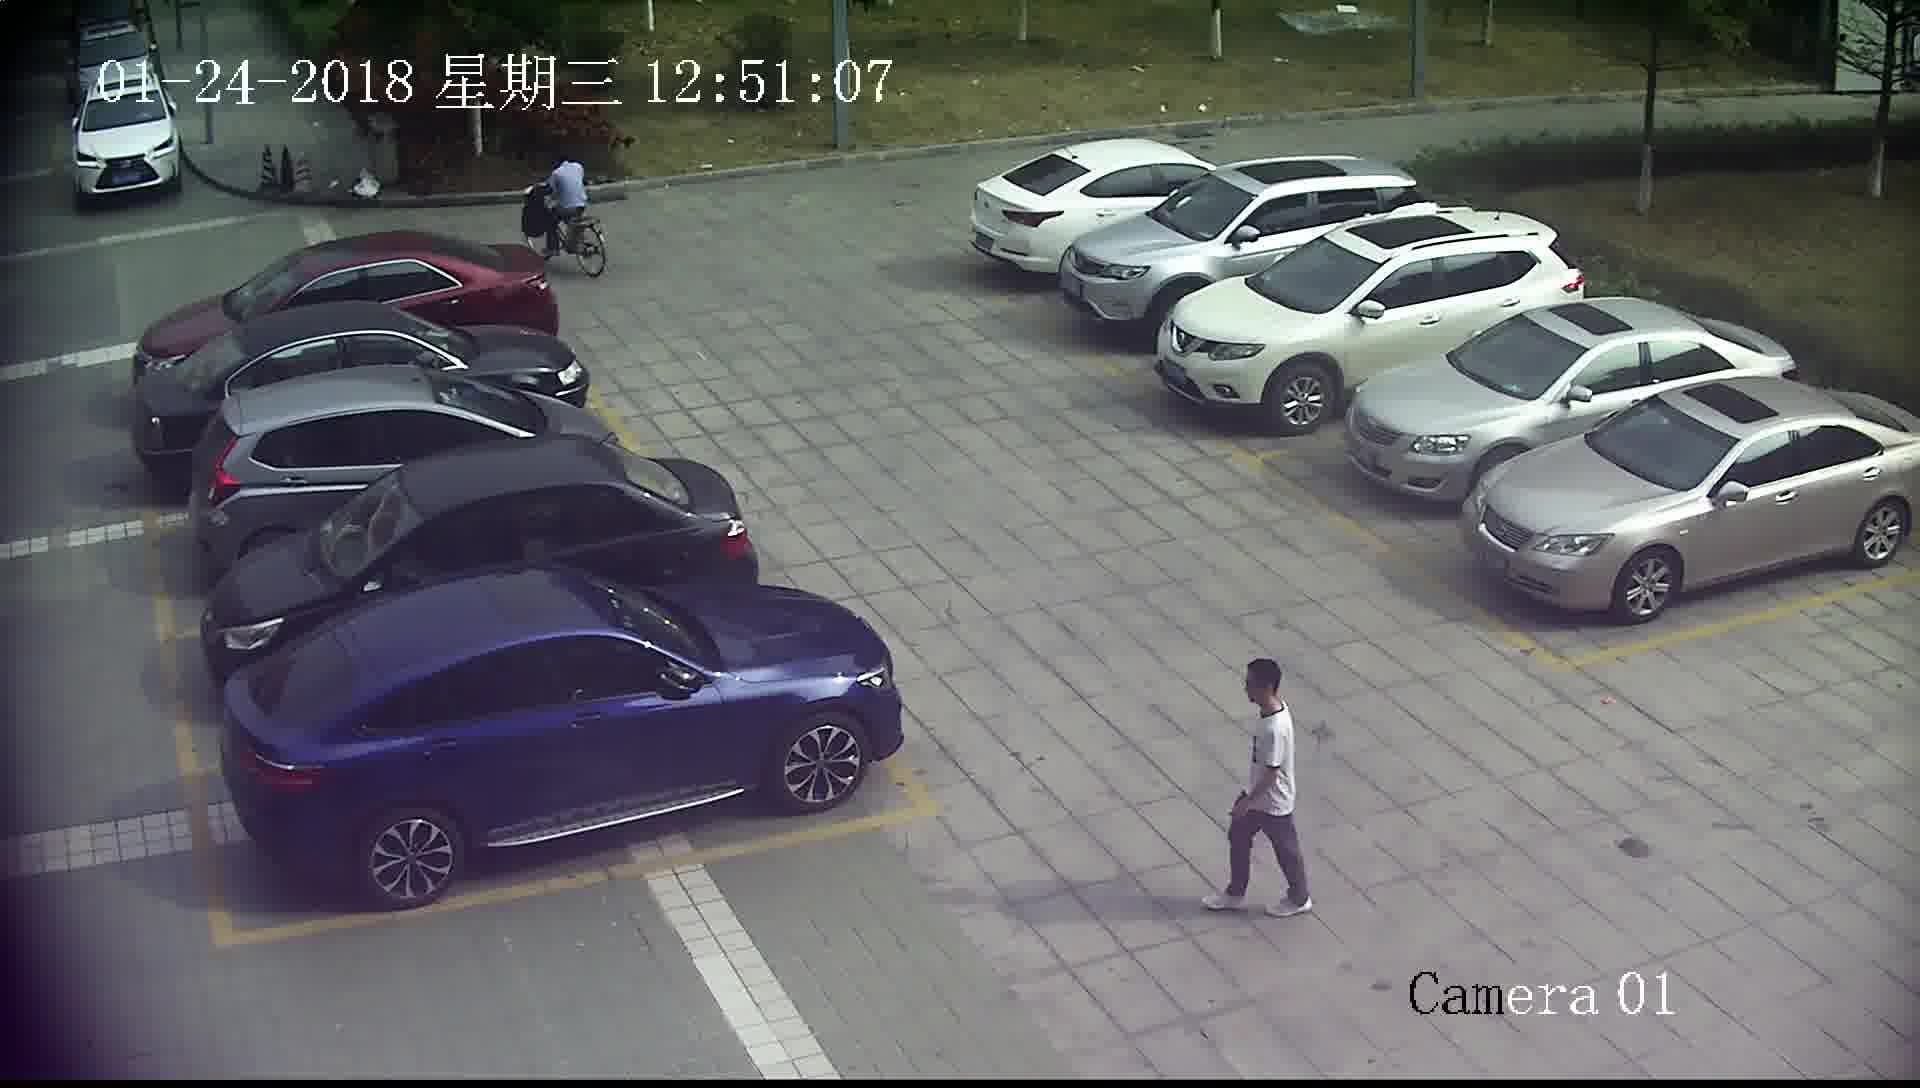
\includegraphics[width=25mm]{1-1}~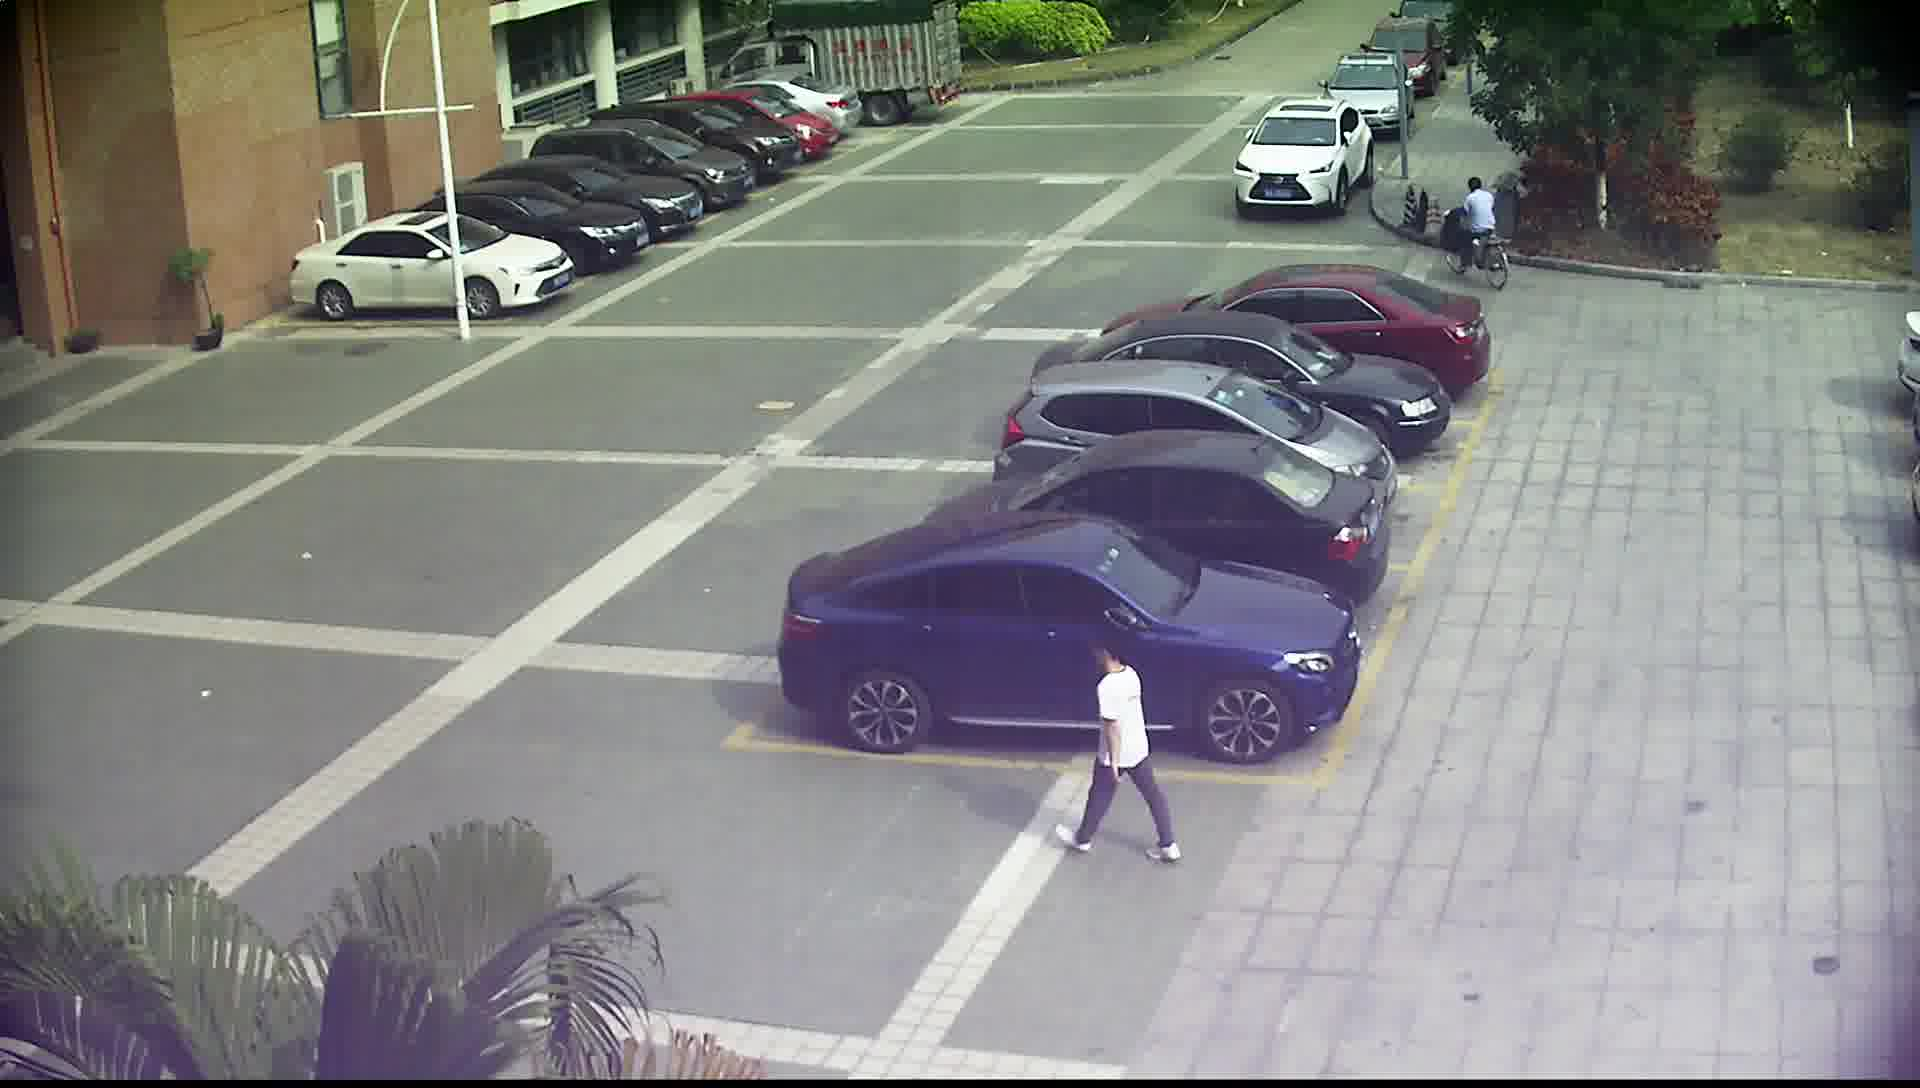
\includegraphics[width=25mm]{1-2} \\
2. 一楼庭院 & 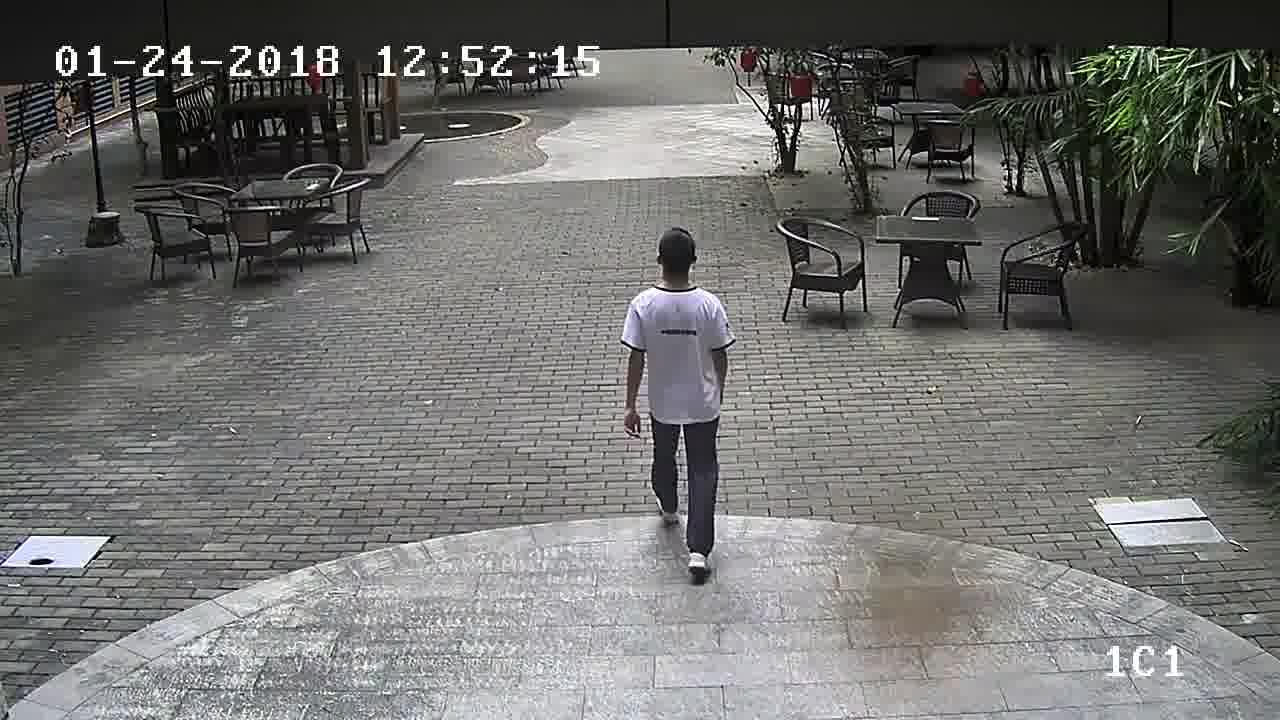
\includegraphics[width=25mm]{1-4}~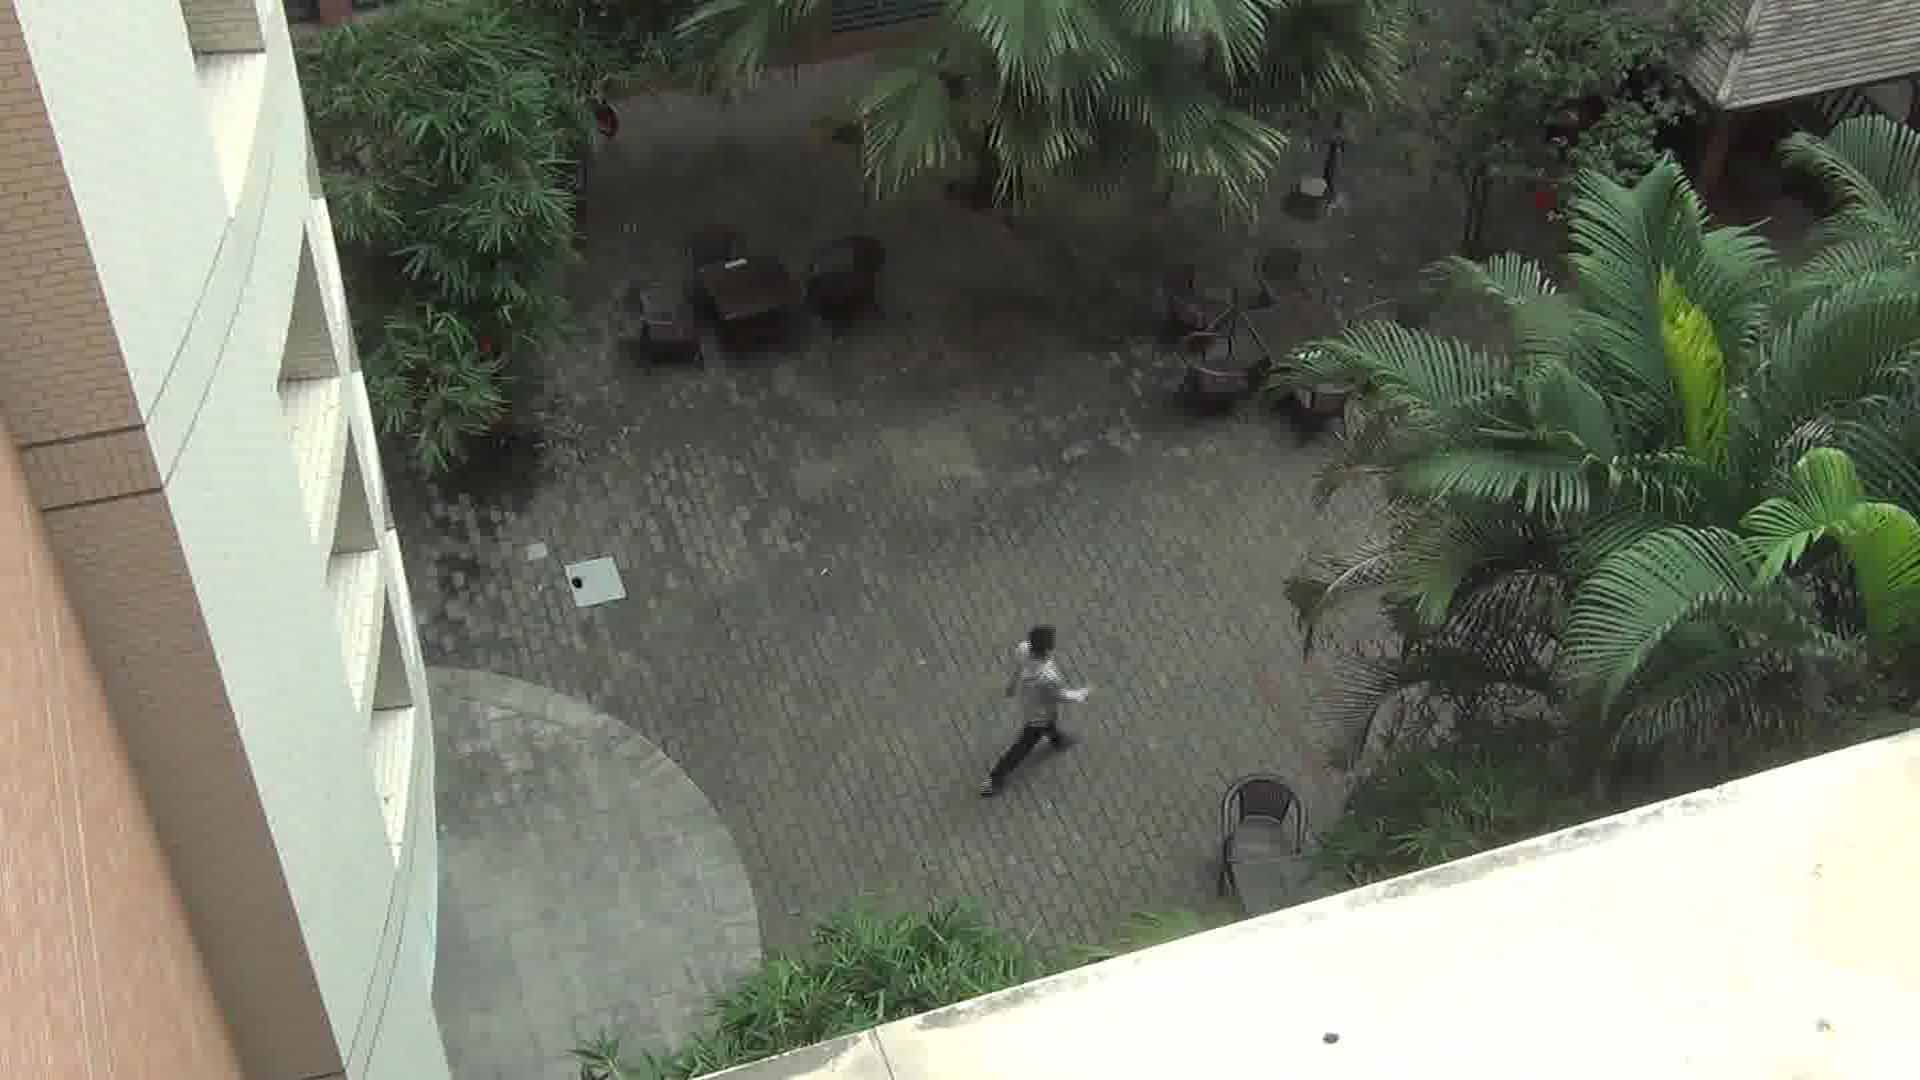
\includegraphics[width=25mm]{1-5}~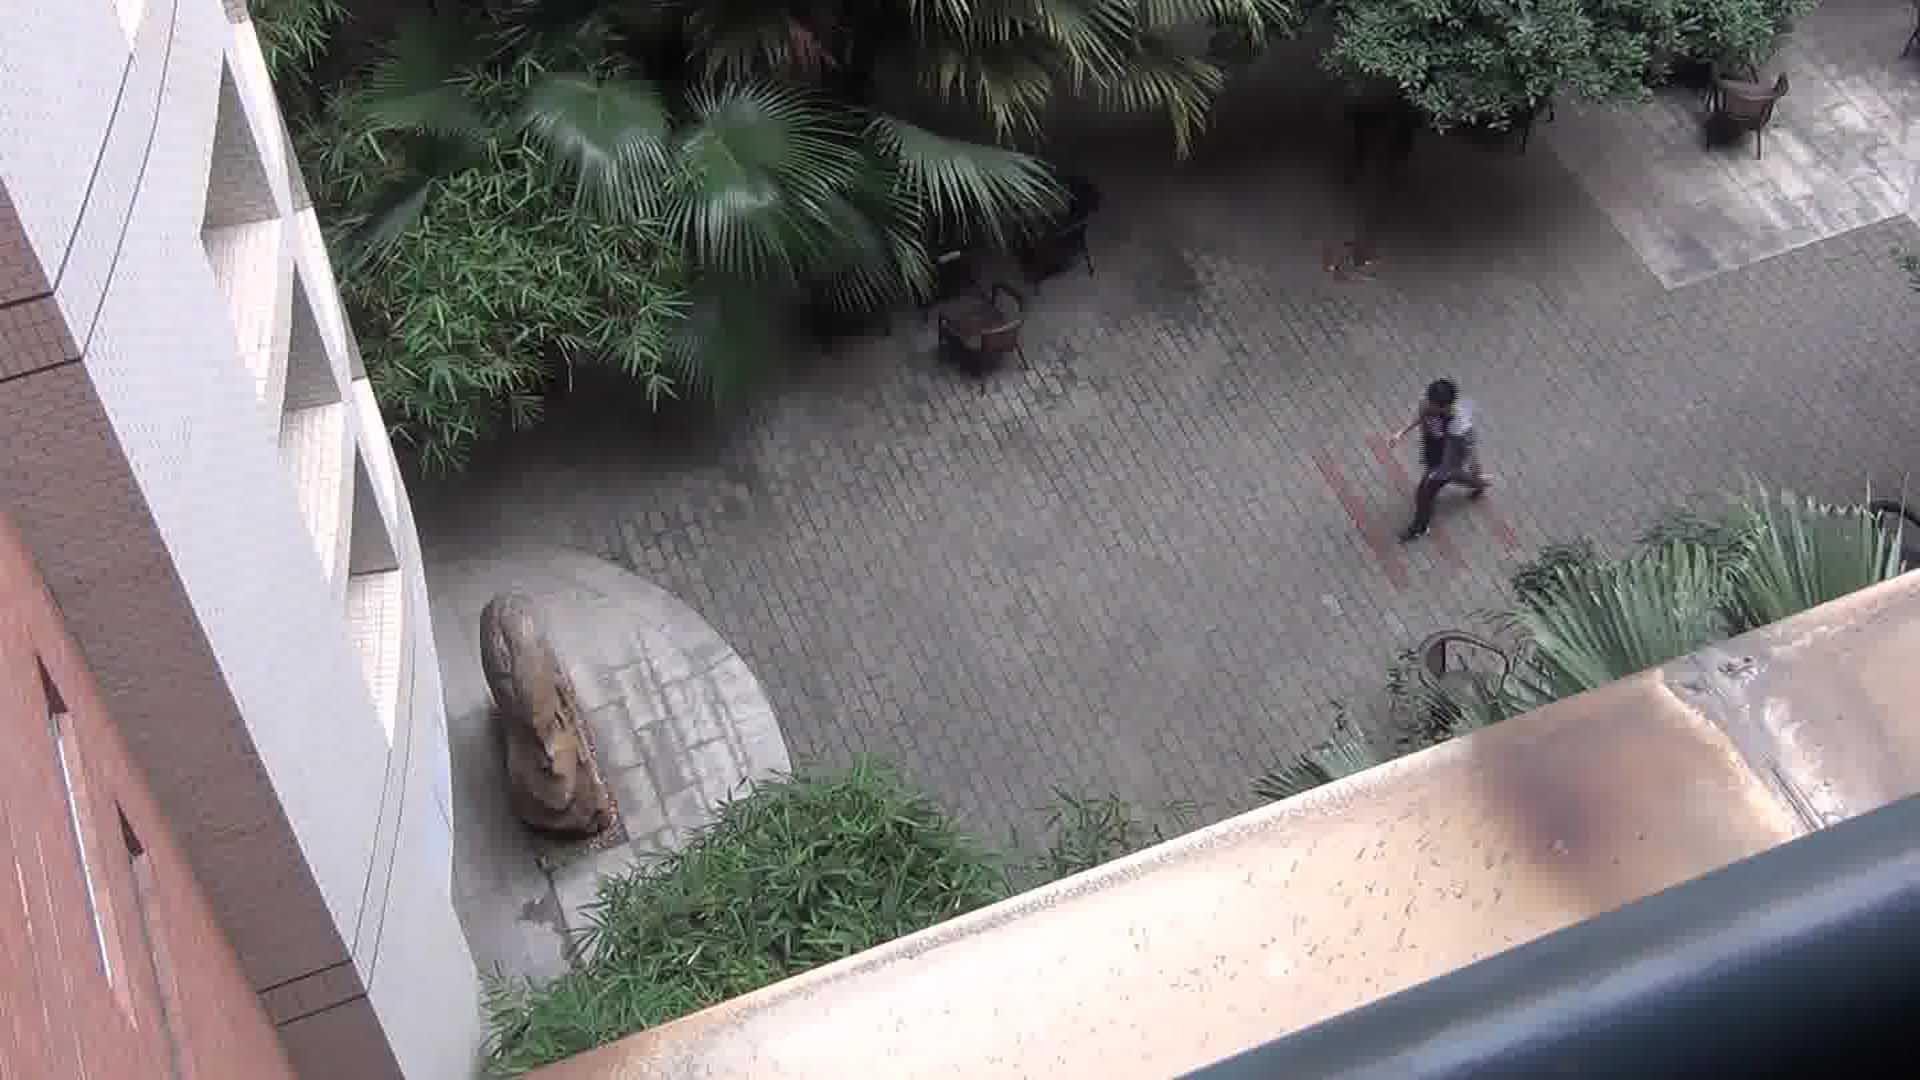
\includegraphics[width=25mm]{1-6} \\
3. 二楼走廊 & 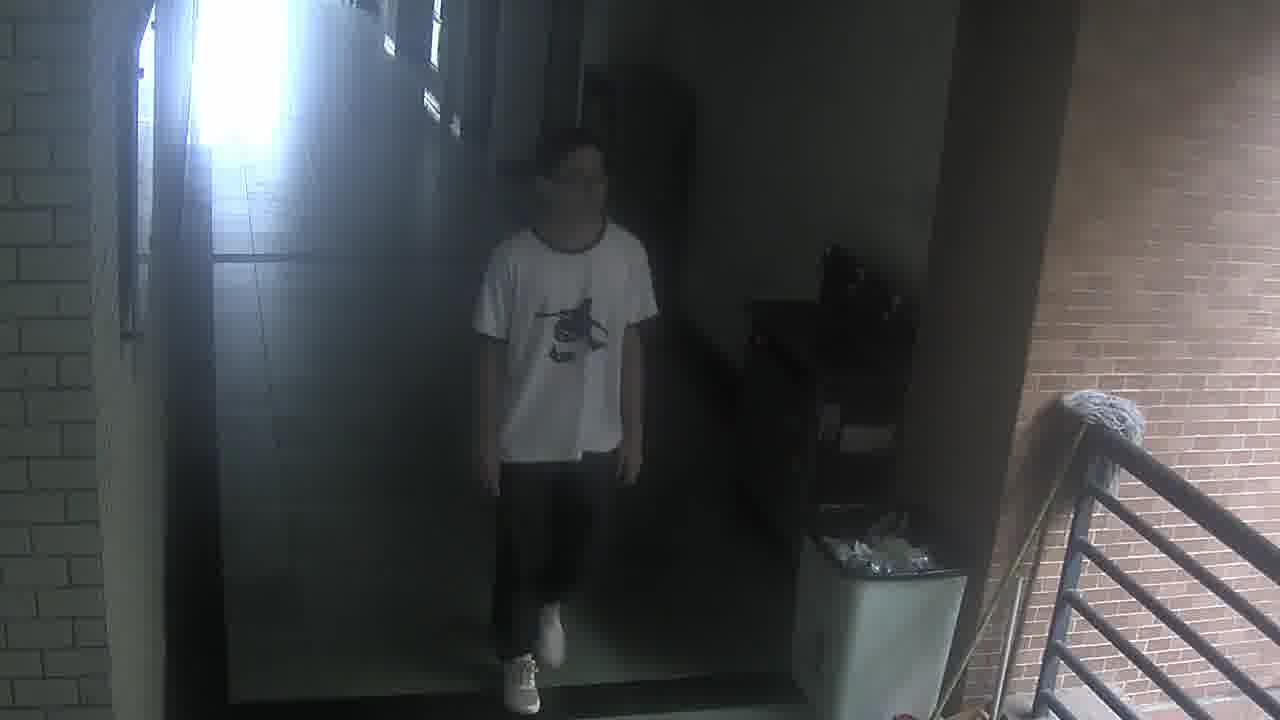
\includegraphics[width=25mm]{2-1}~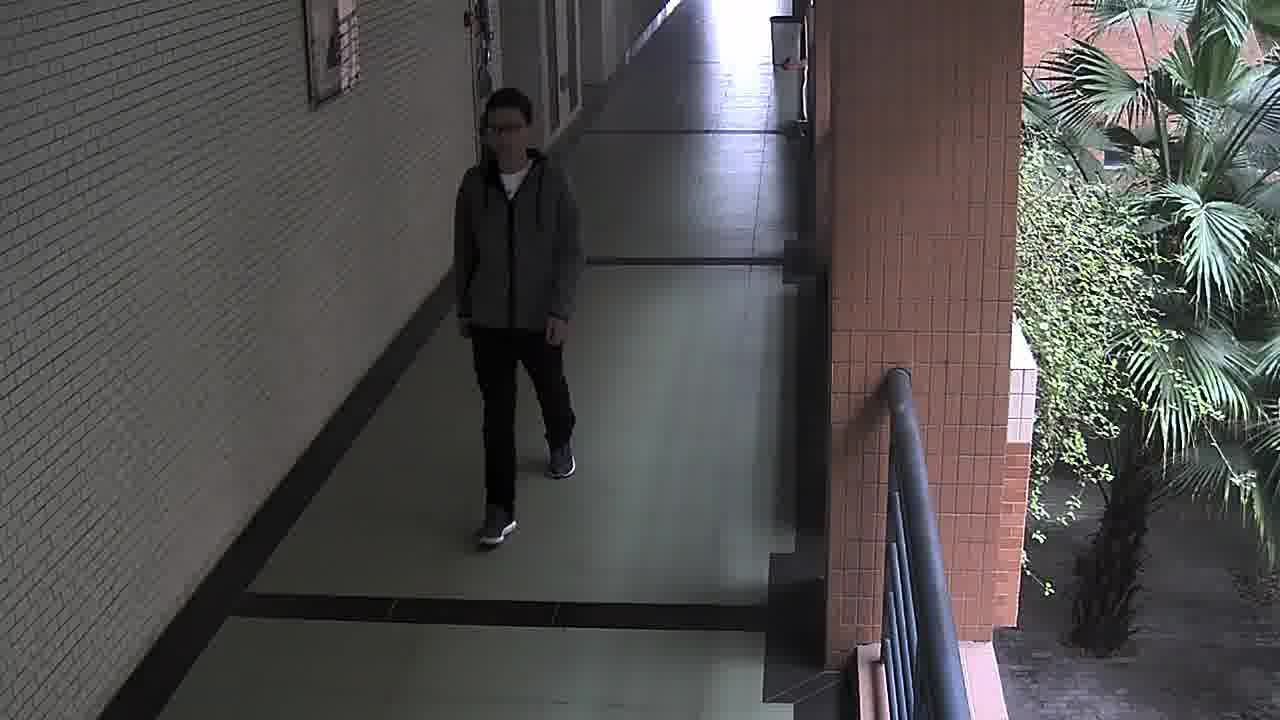
\includegraphics[width=25mm]{2-2}~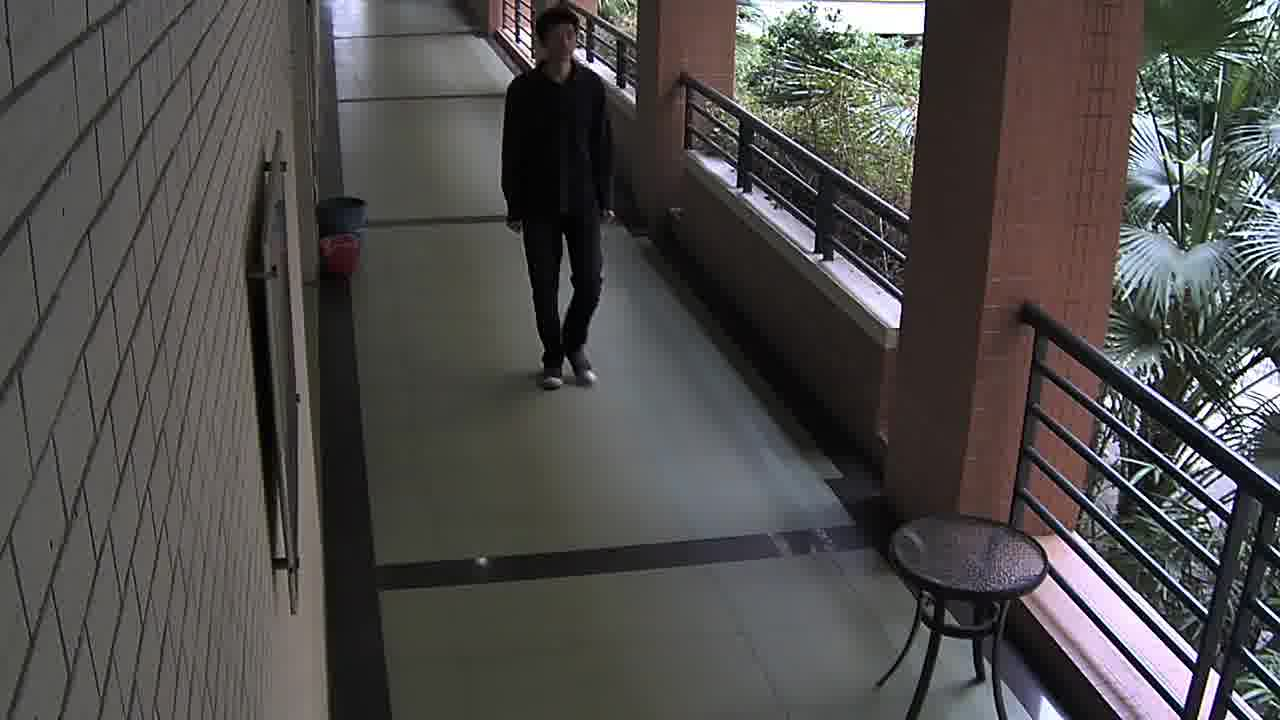
\includegraphics[width=25mm]{2-3}~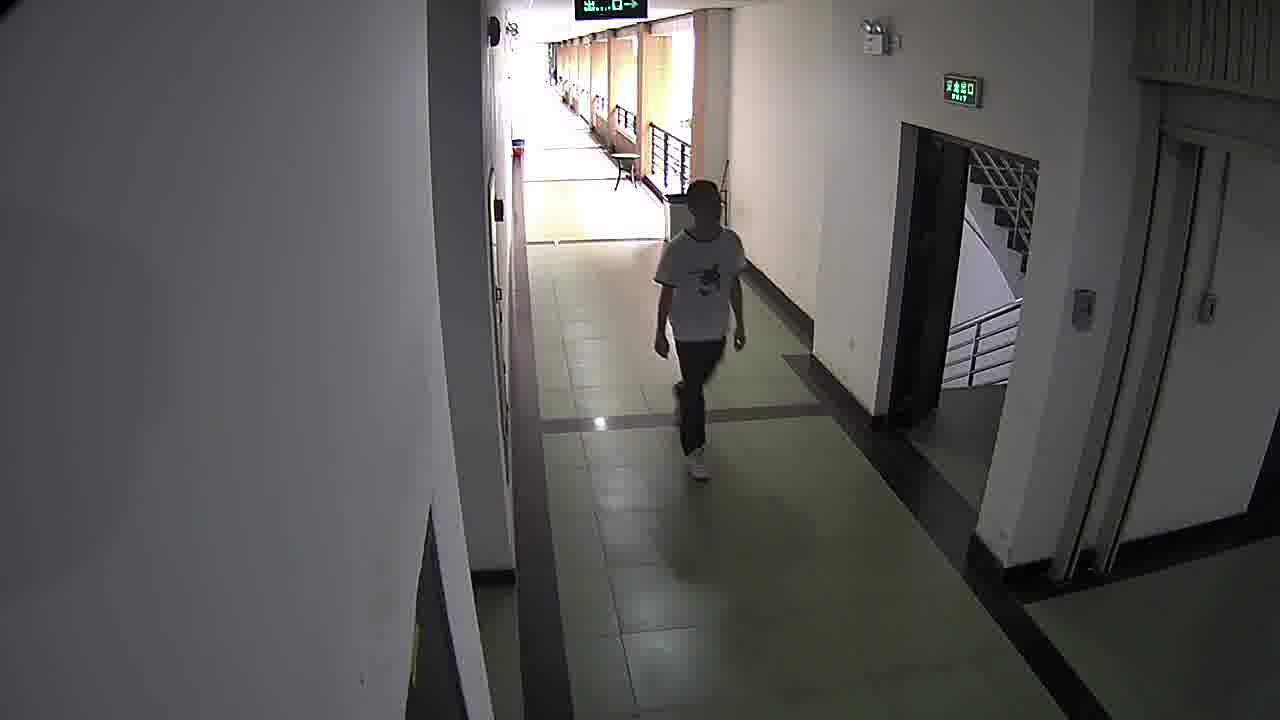
\includegraphics[width=25mm]{2-4} \\
4. 三楼电梯 & 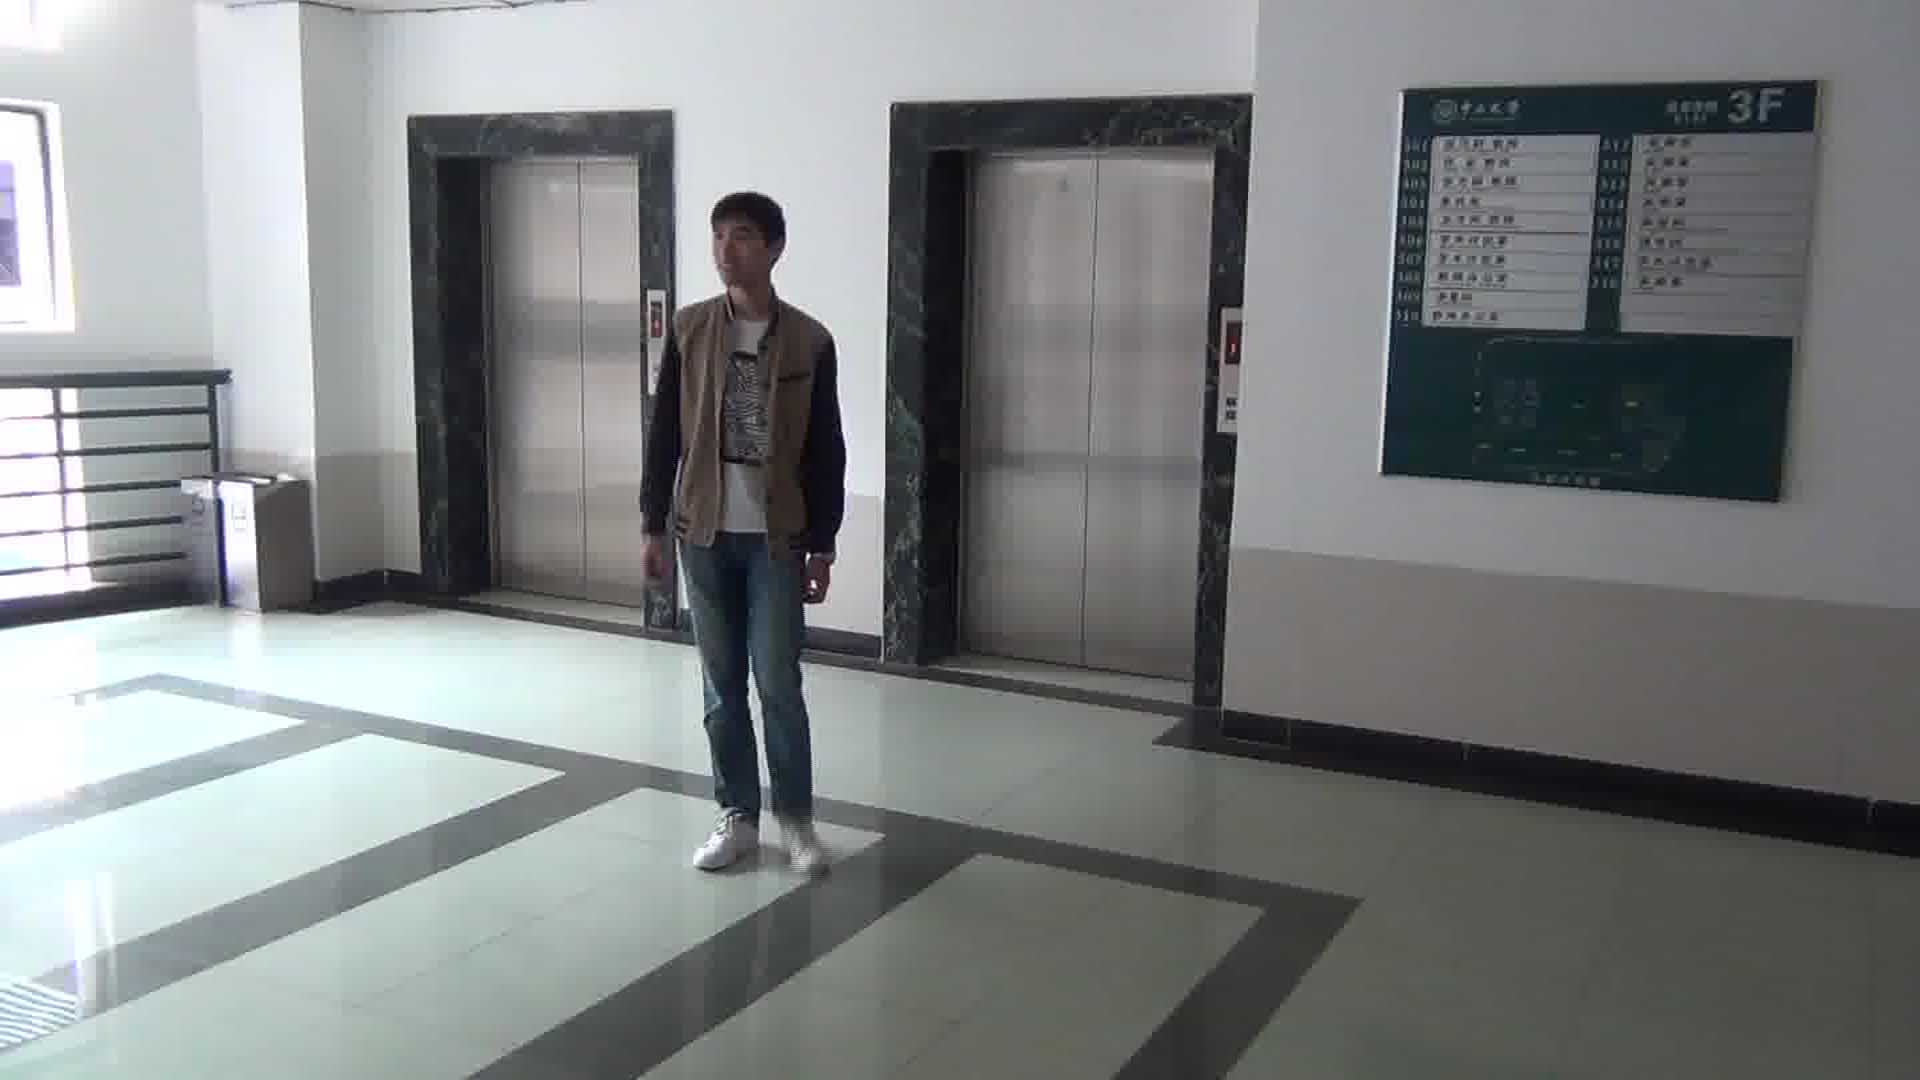
\includegraphics[width=25mm]{3-1}~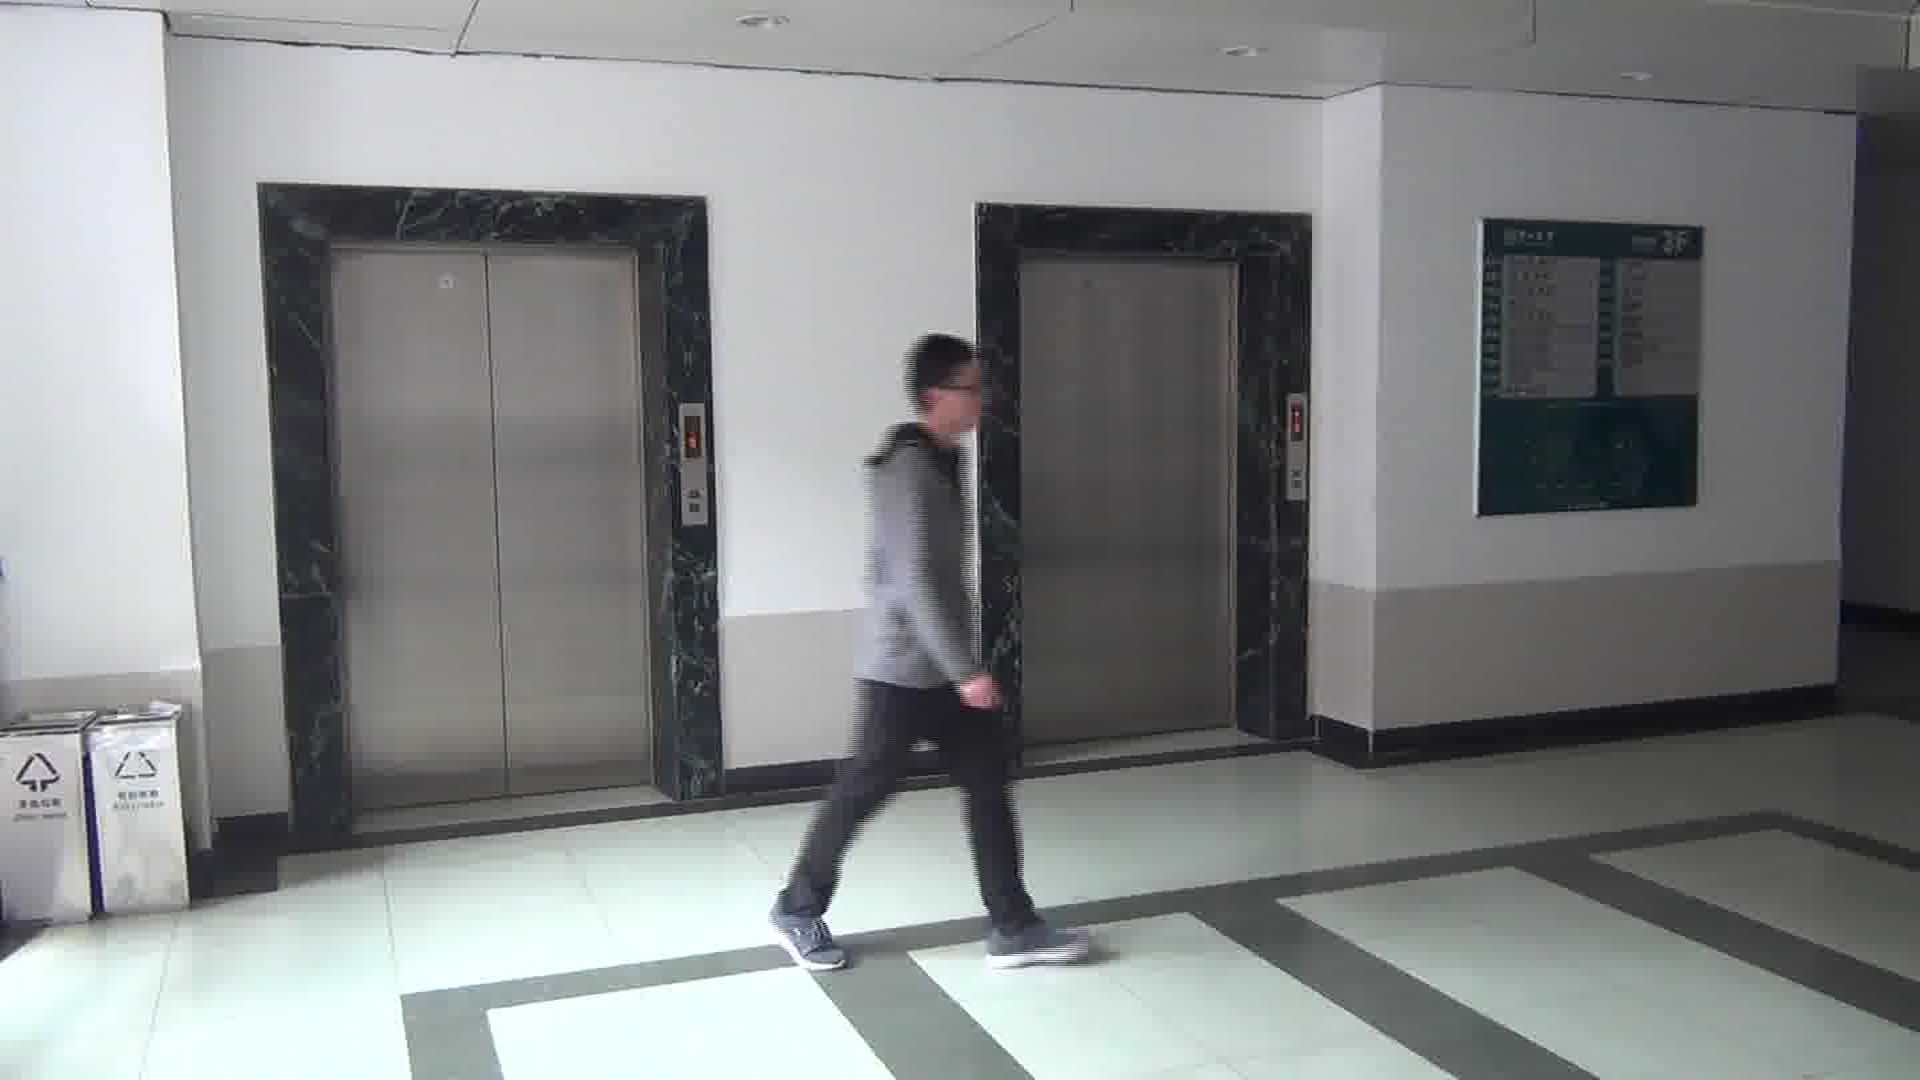
\includegraphics[width=25mm]{3-2}~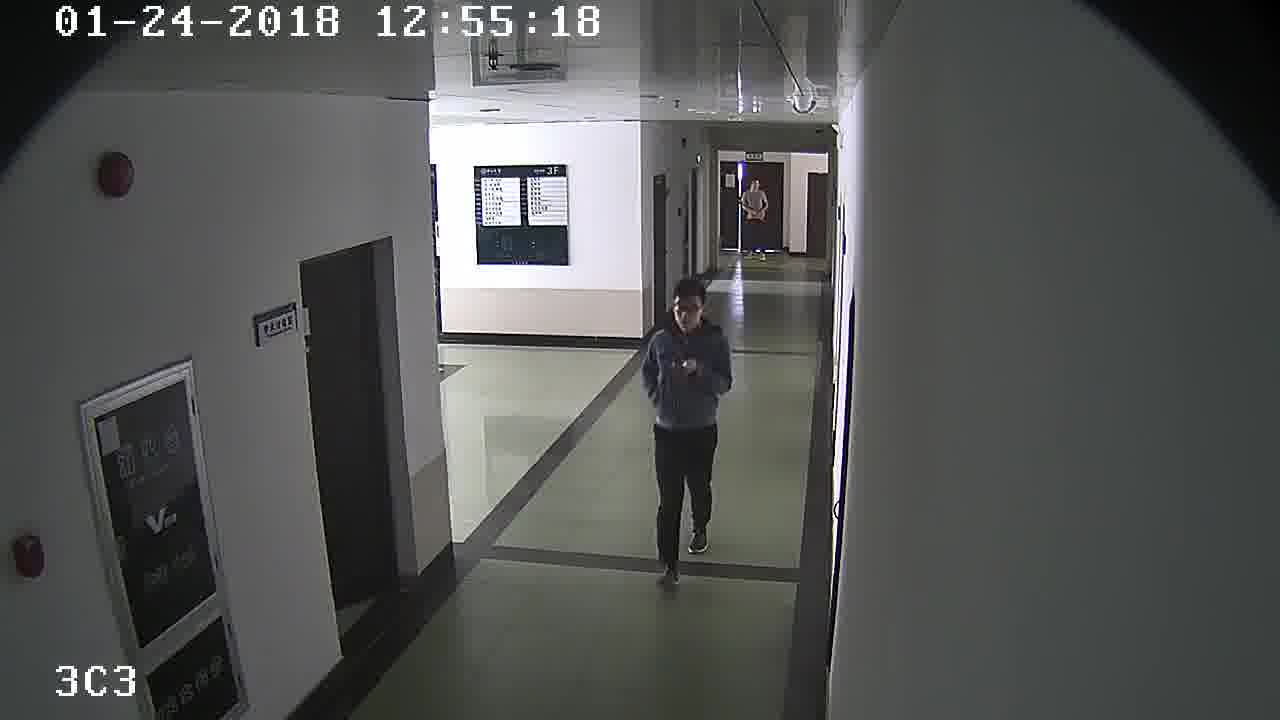
\includegraphics[width=25mm]{3-3} \\
5. 三楼走廊 & 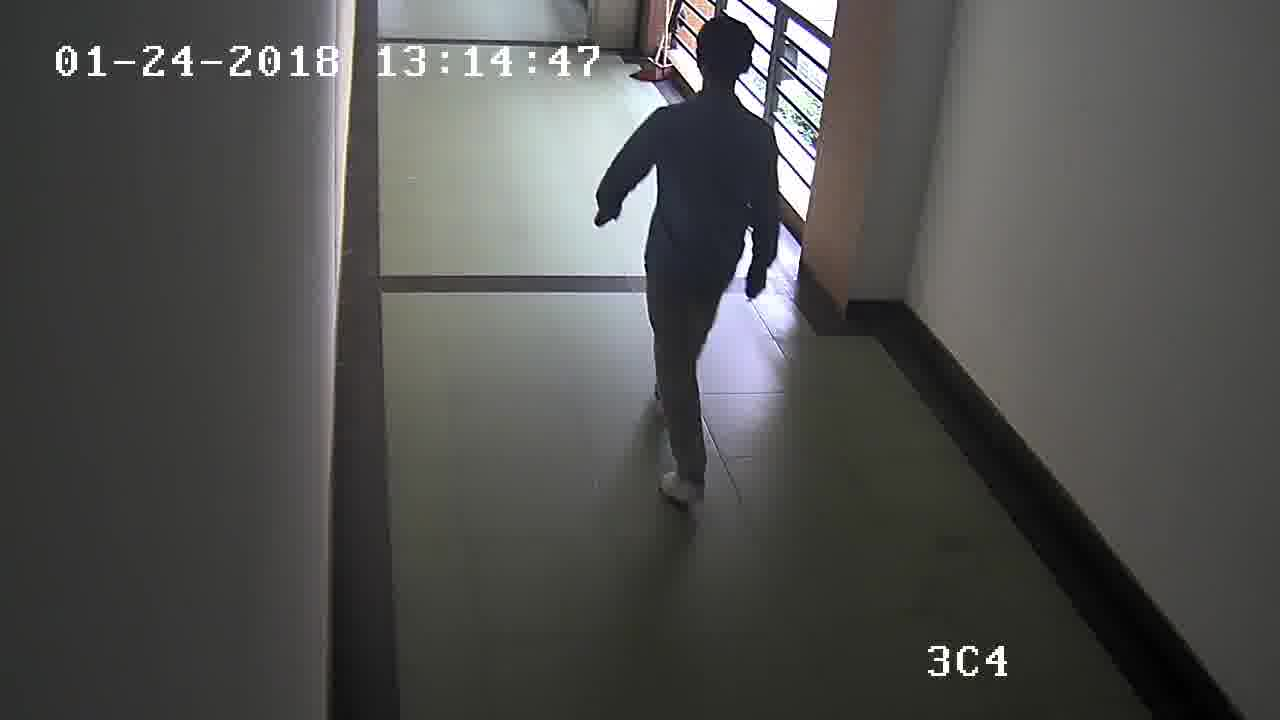
\includegraphics[width=25mm]{3-4}~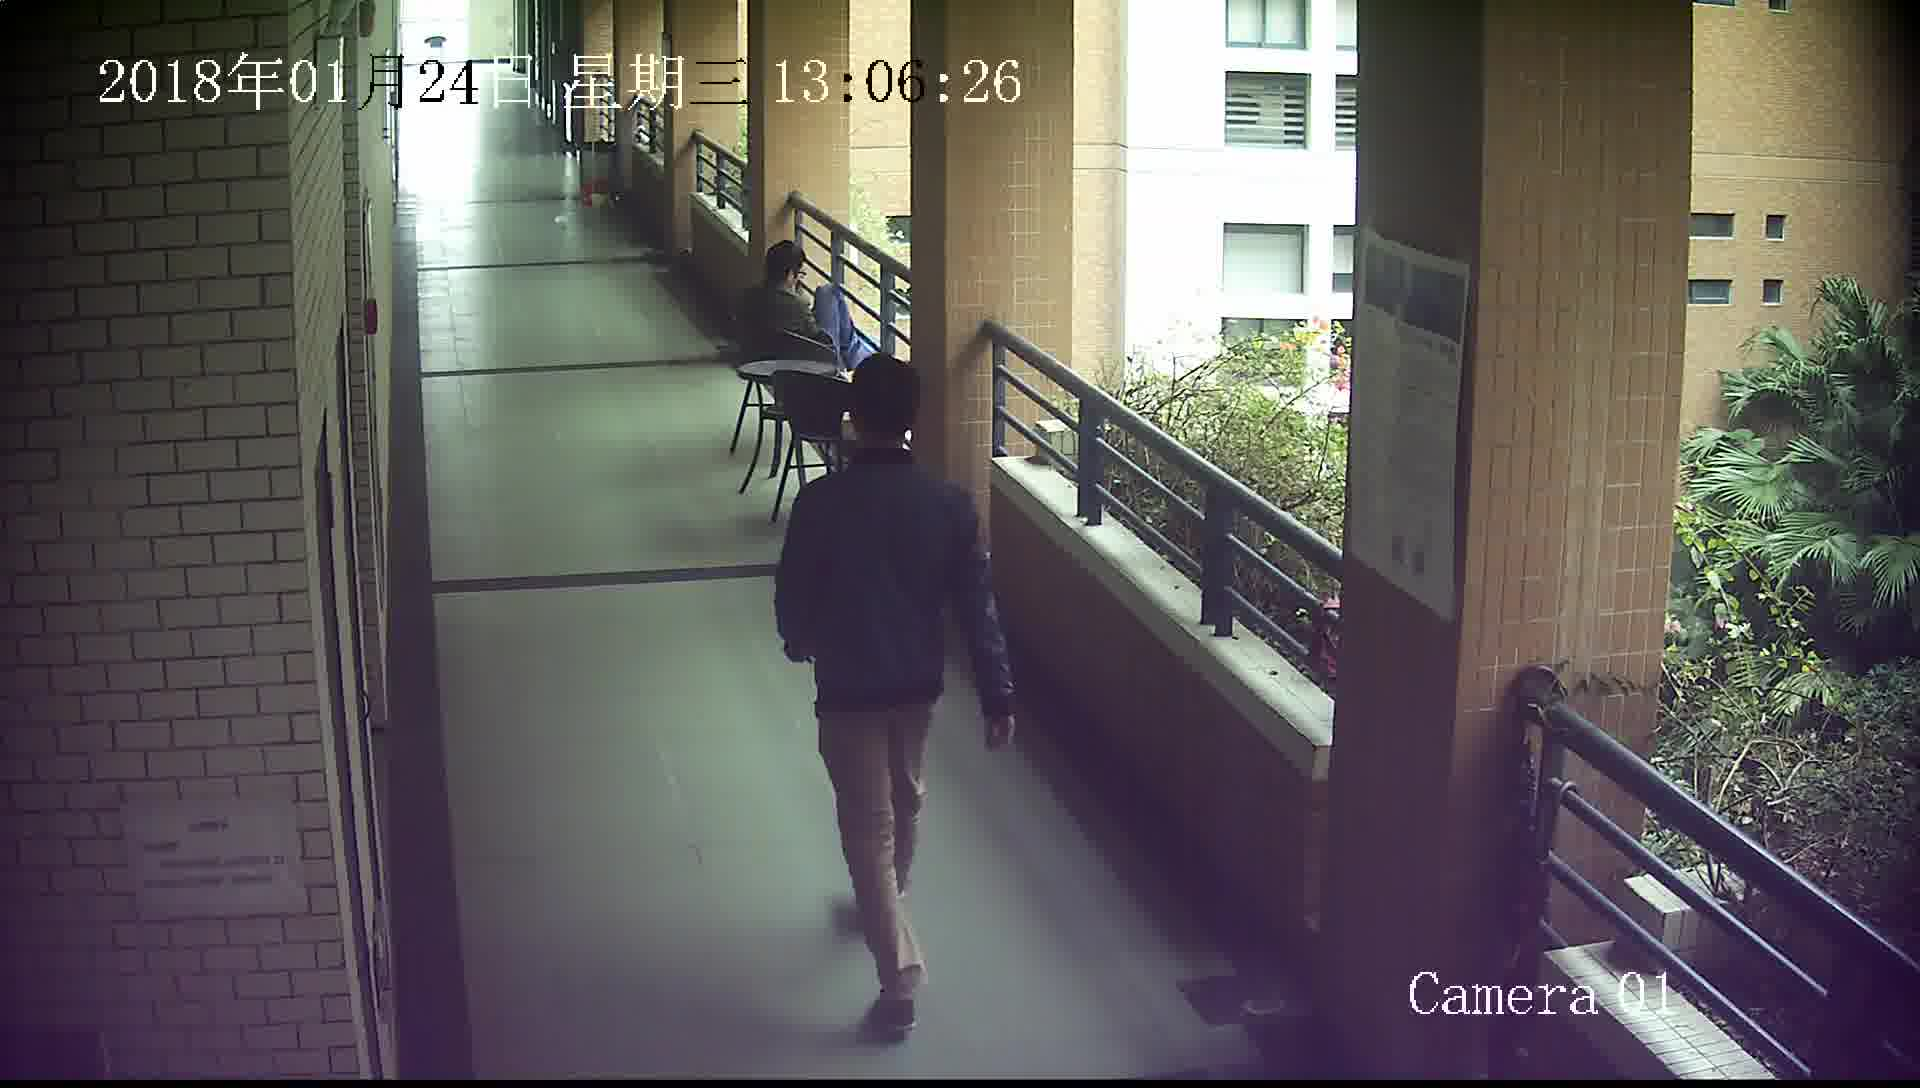
\includegraphics[width=25mm]{3-5}~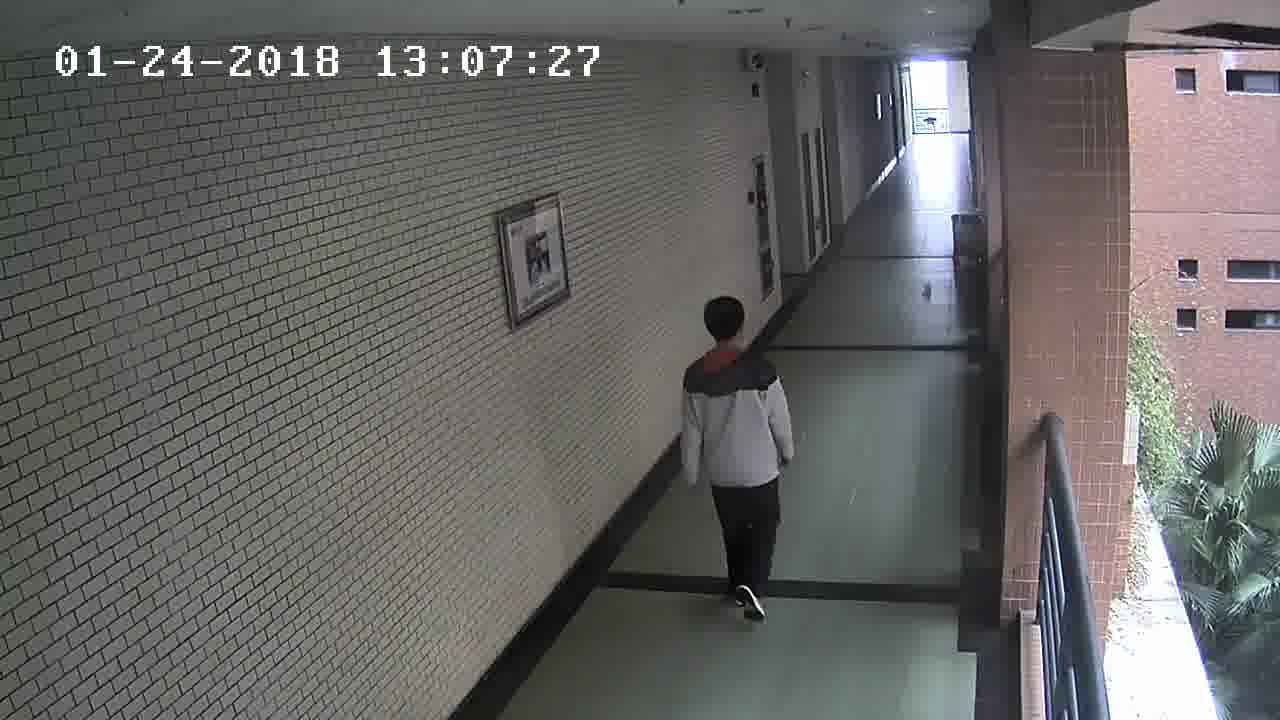
\includegraphics[width=25mm]{3-6}~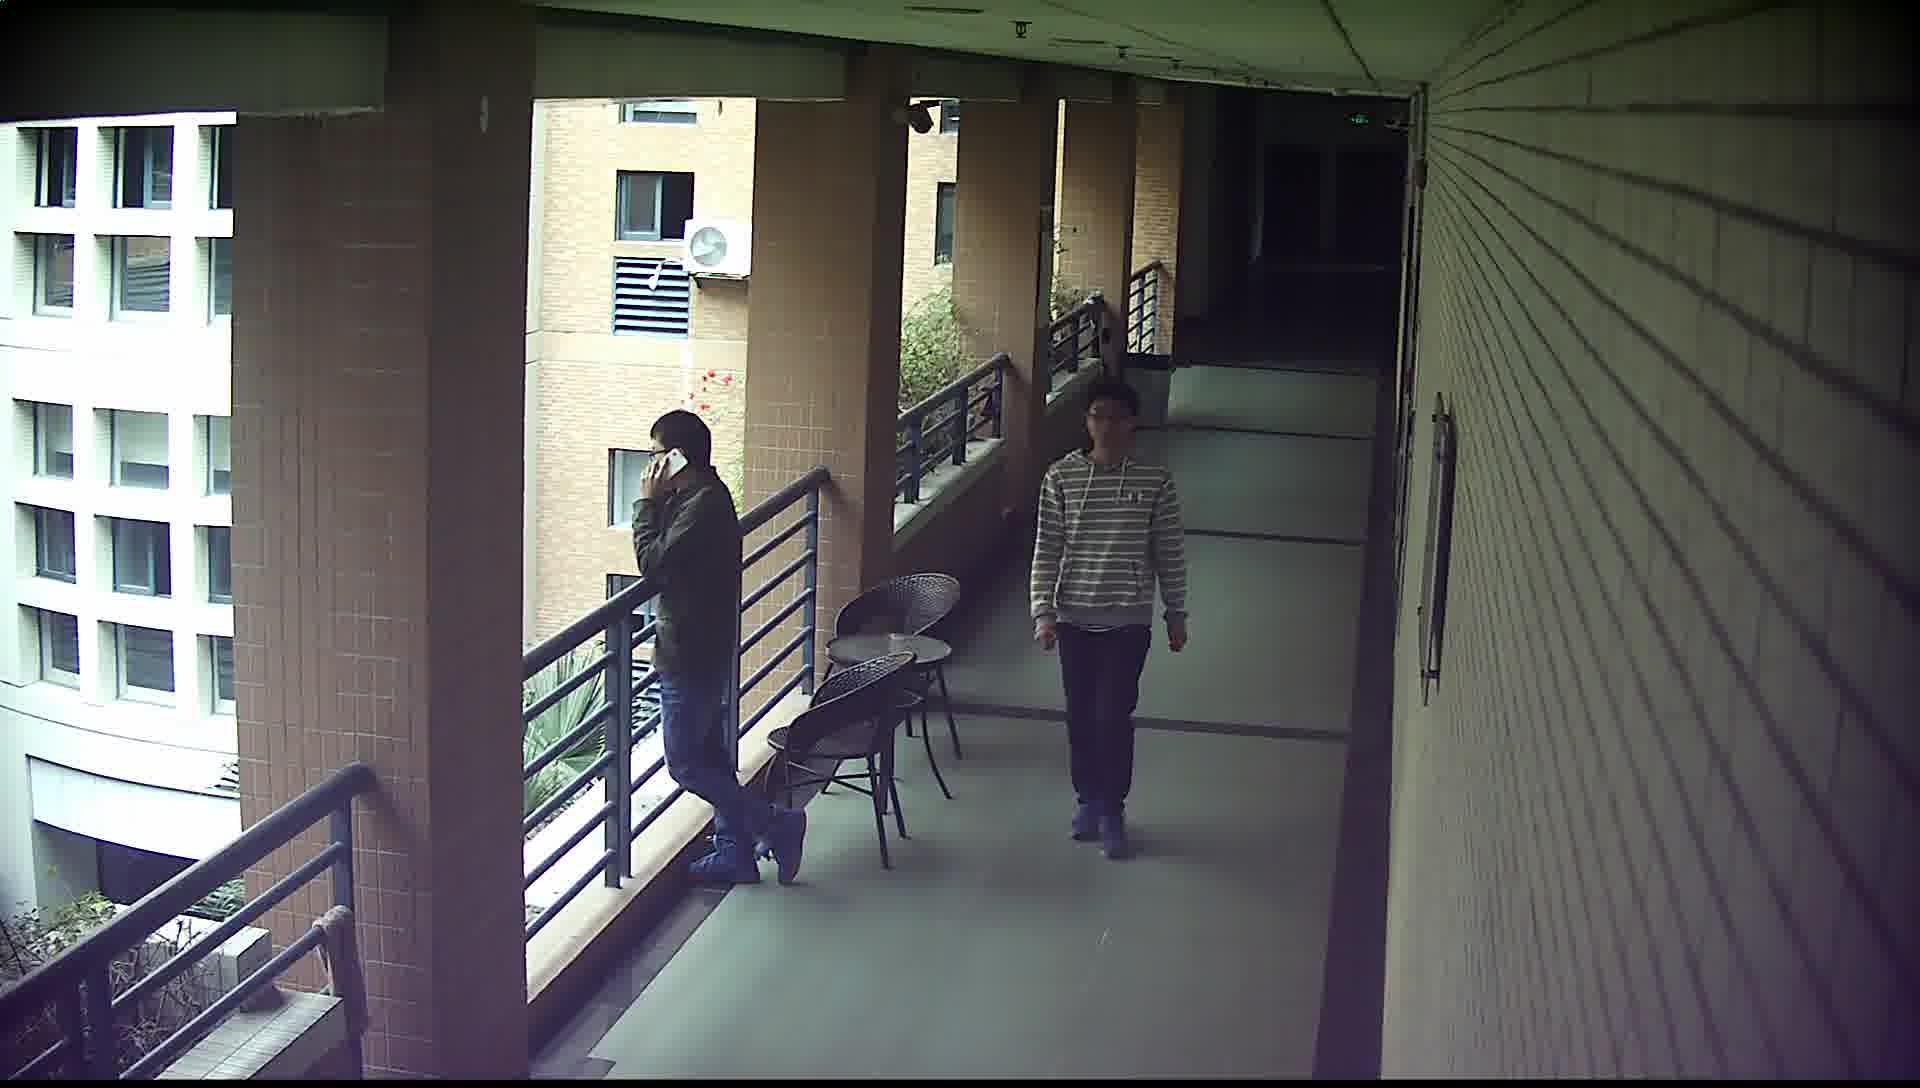
\includegraphics[width=25mm]{3-7} \\
\bottomrule
\end{tabularx}
\end{table}
第5组场景三楼走廊也有类似情况,第1个摄像头的视野很窄,行人能够在很短时间内通过画面,而第4个摄像头则几乎能把行人通过走廊的整个过程记录下来。

\subsection{行人检测效果及人工标注结果}

行人检测使用了Detectron工具,由于Detectron实现了Mask RCNN,所以可以将行人的轮廓分割出来。图\ref{fig:detectron}展示了行人检测可视化的效果。

\begin{figure}
\centering
\subfloat[场景1]{\centering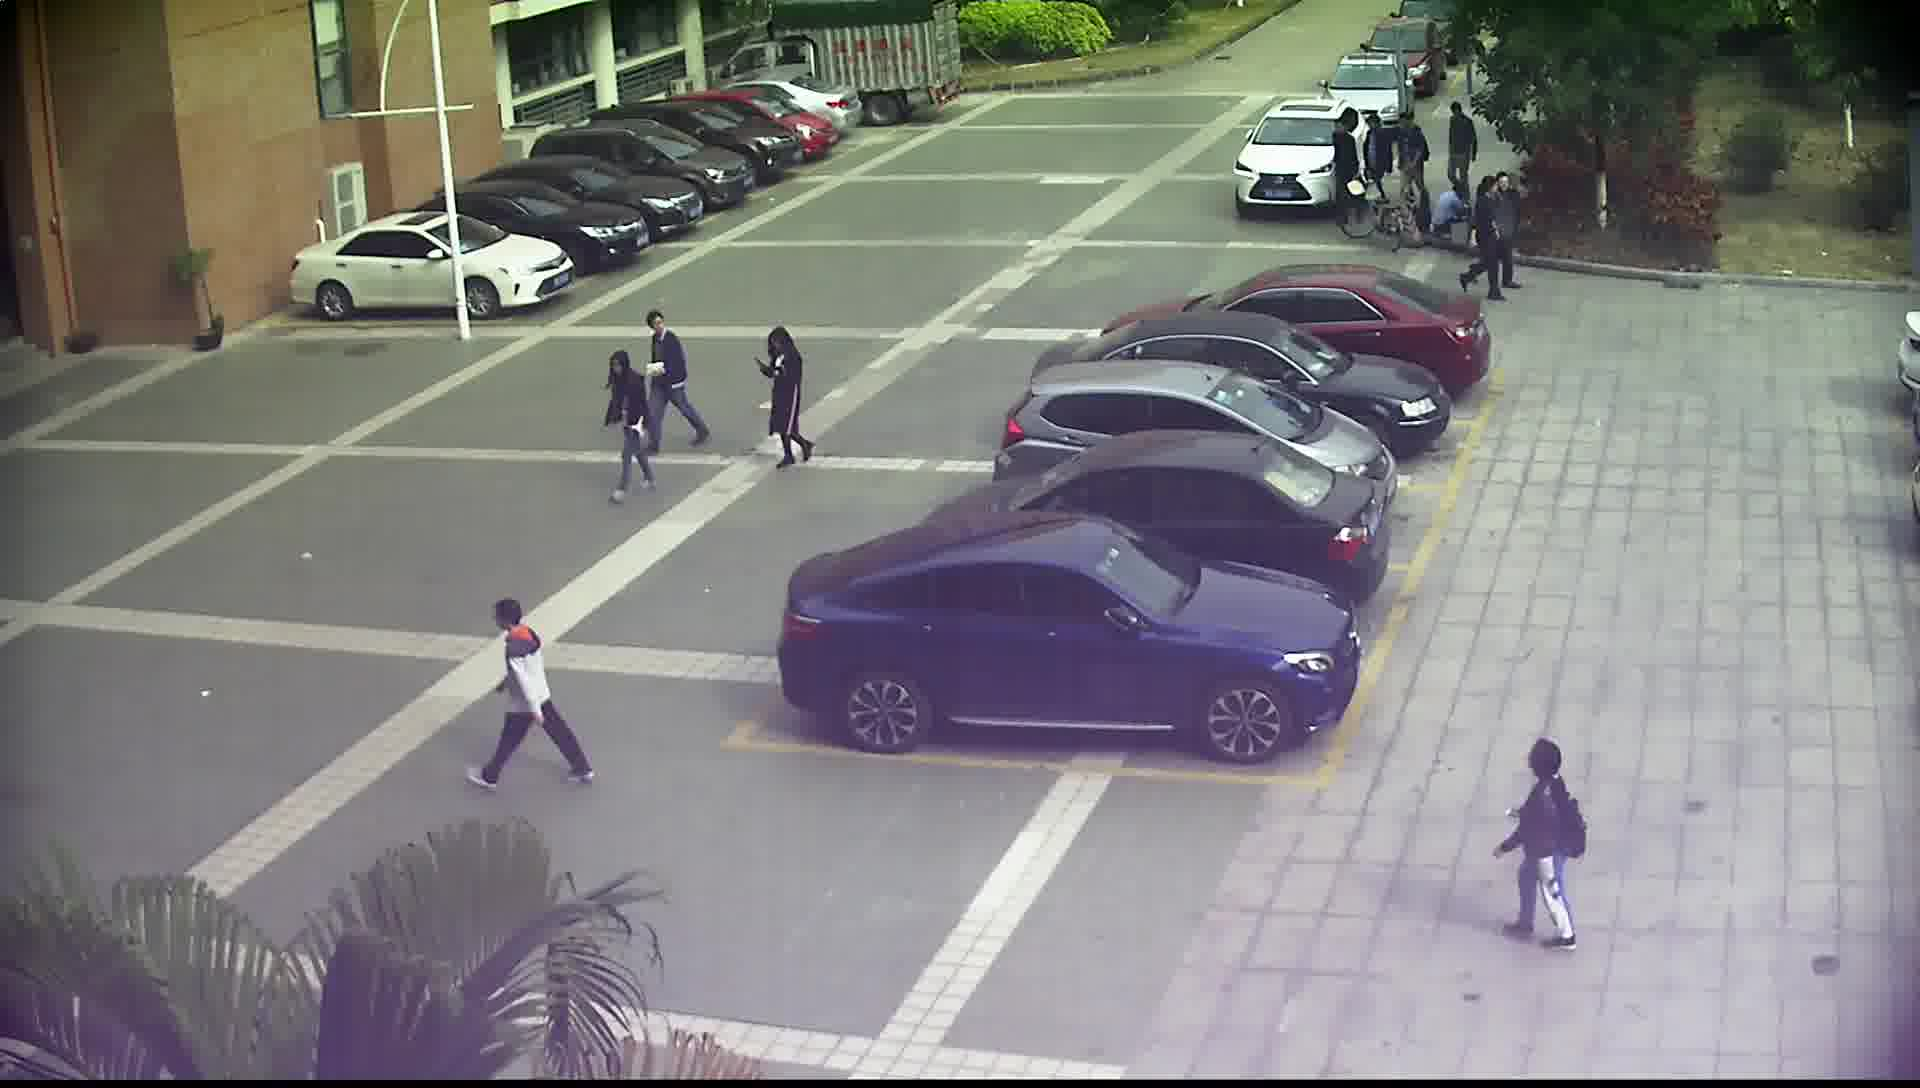
\includegraphics[width=0.4\textwidth]{1-2_5_151}}\quad
\subfloat[场景2]{\centering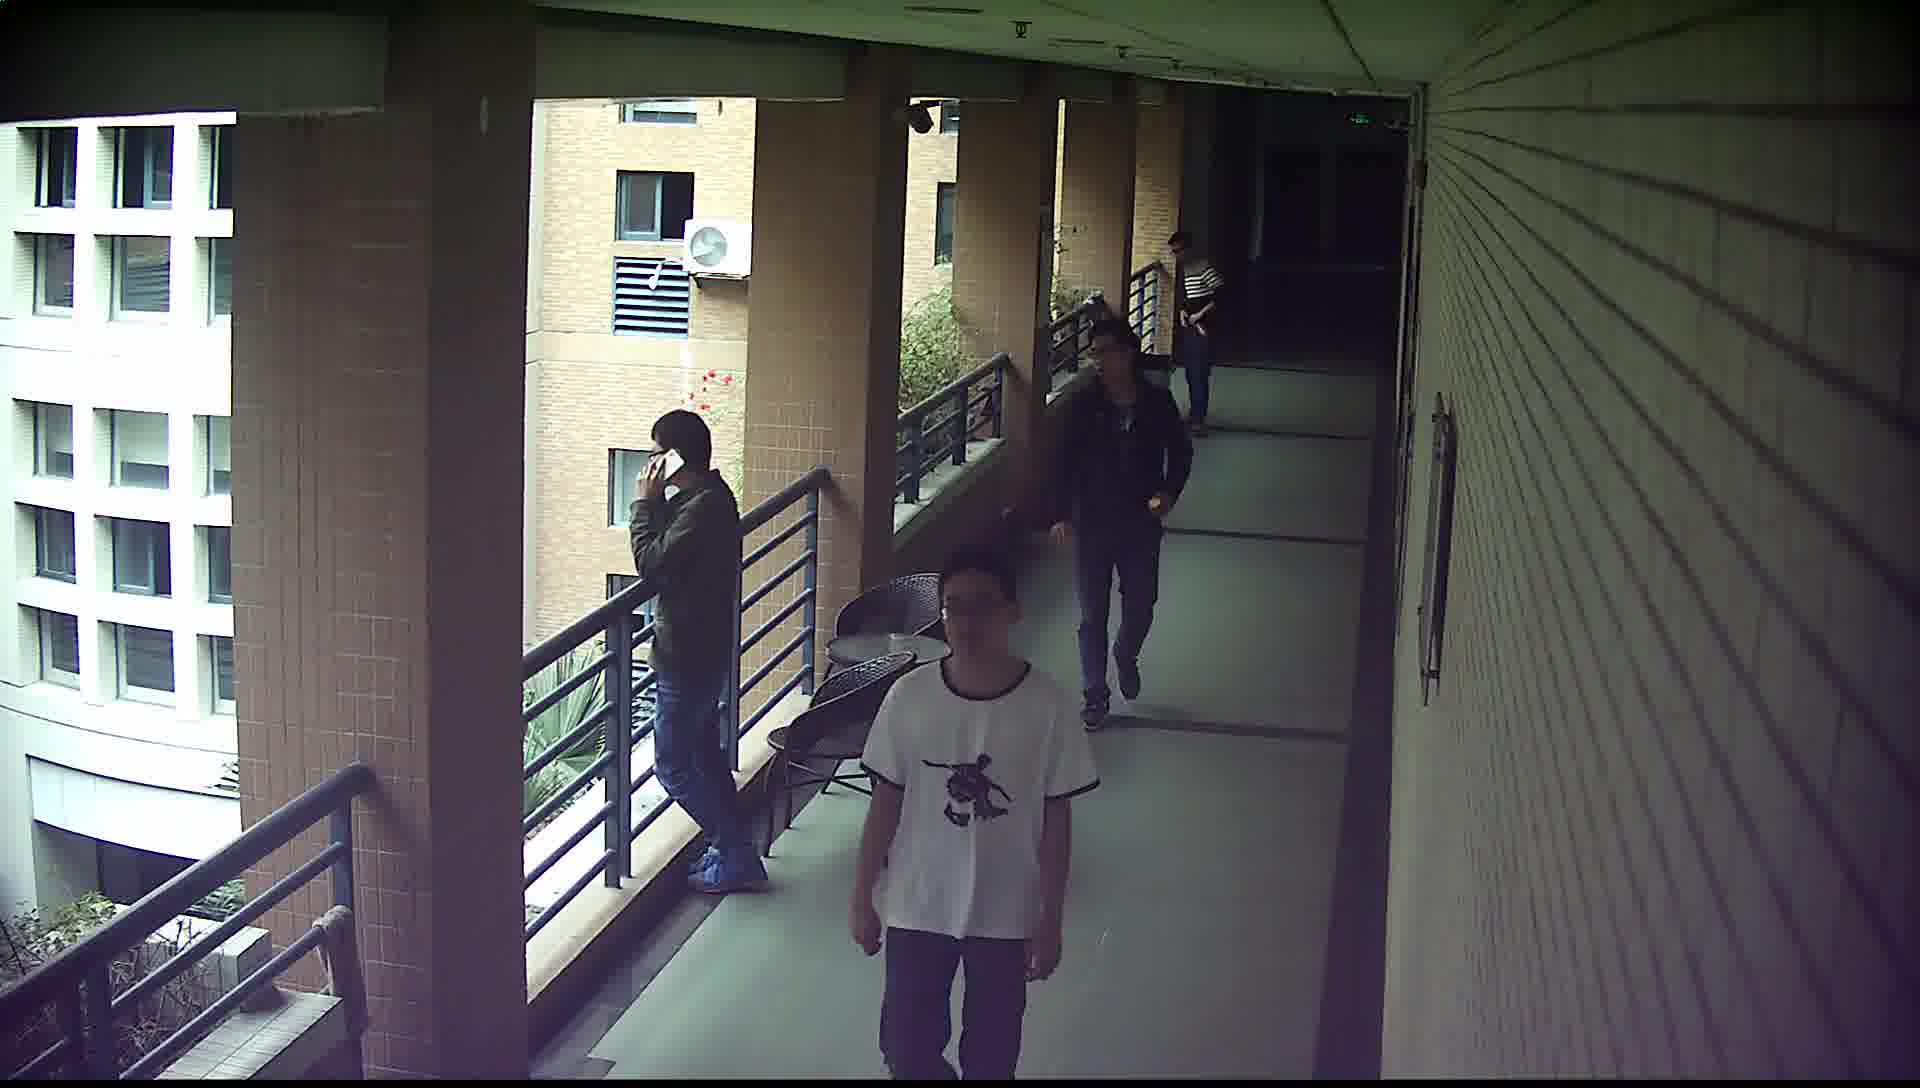
\includegraphics[width=0.4\textwidth]{3-7_10_394}}\\
\subfloat[场景1检测结果]{\centering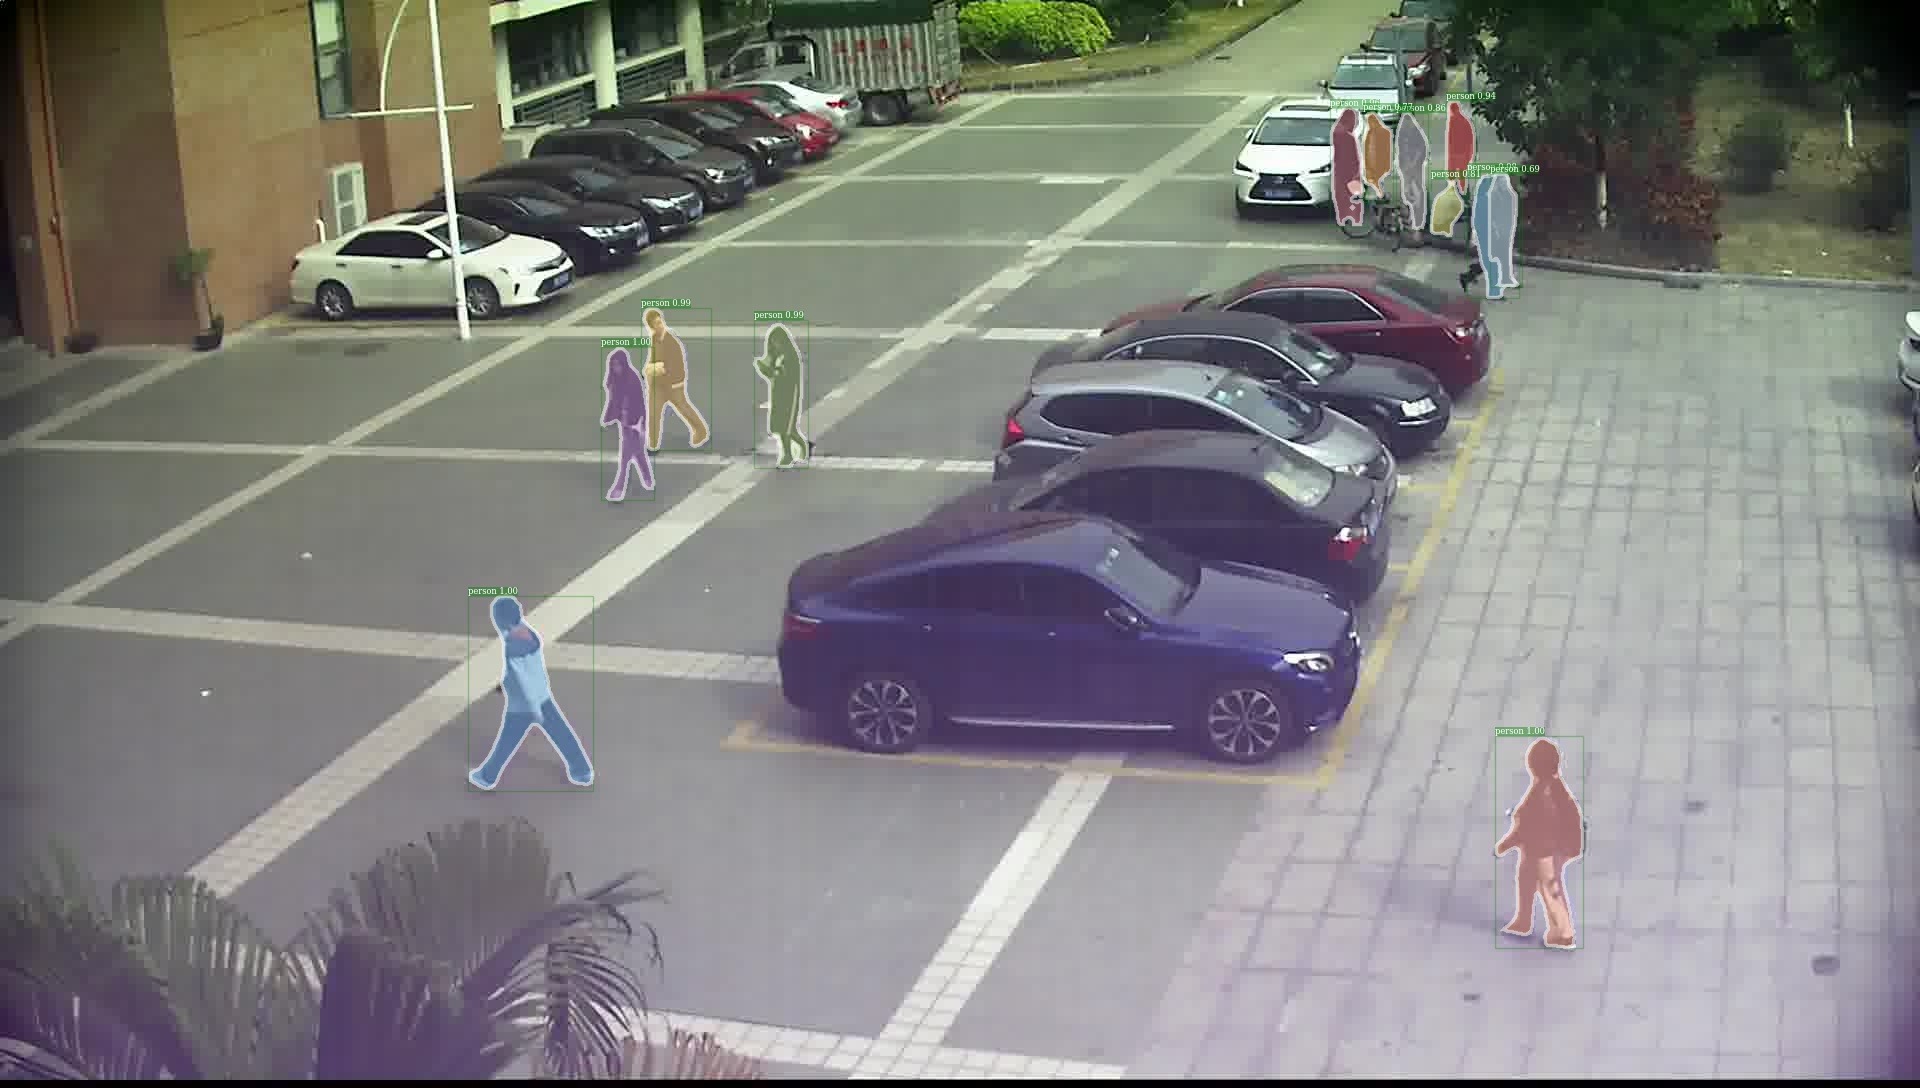
\includegraphics[width=0.4\textwidth]{1-2_5_151_det}}\quad
\subfloat[场景2检测结果]{\centering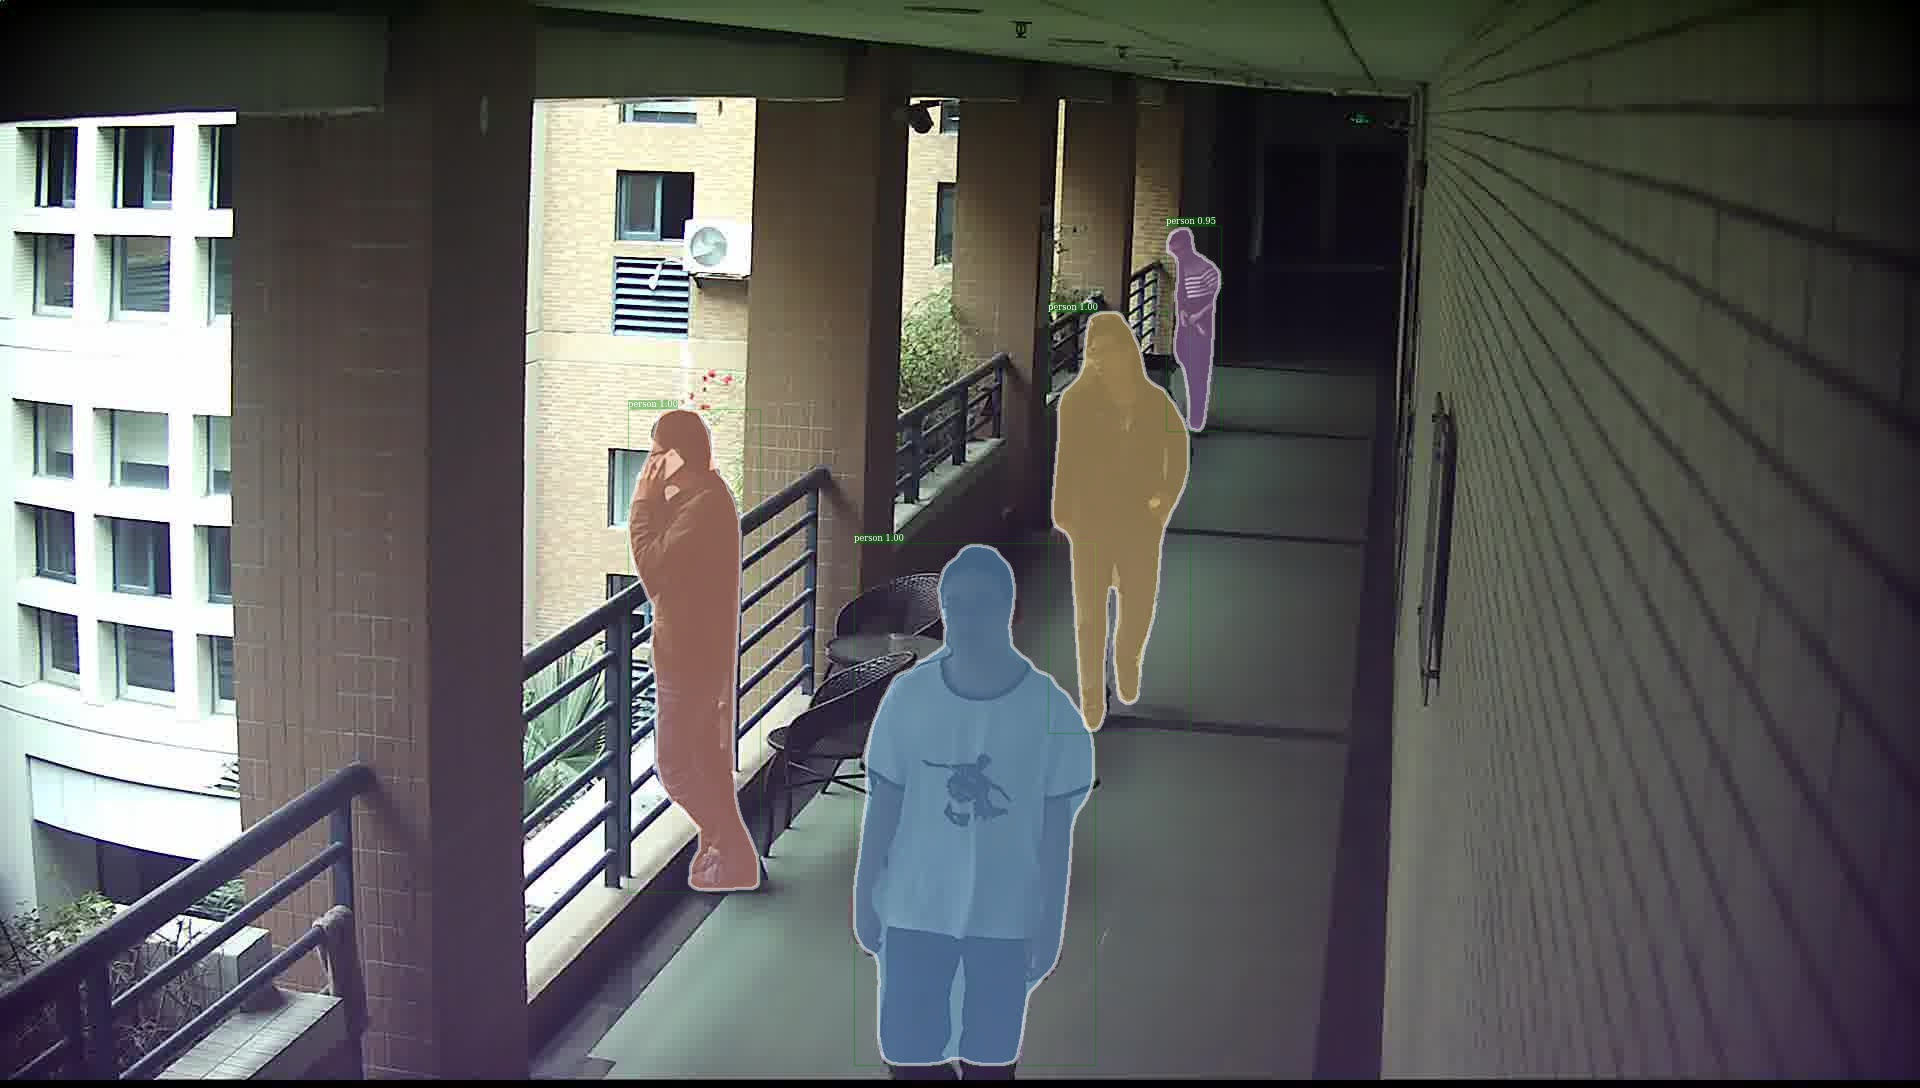
\includegraphics[width=0.4\textwidth]{3-7_10_394_det}}
\caption{Detectron行人检测结果可视化}
\label{fig:detectron}
\end{figure}

图\ref{fig:label}展示了经过人工标注后得到的同一行人在不同摄像头下的图片。从图中可以看出,同一行人在不同的视角下,差距很大,对于行人重识别算法以及人物跟踪任务极具挑战性。

\begin{figure}
\centering
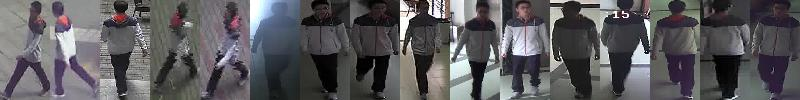
\includegraphics[width=\textwidth]{label}
\caption{同一行人在不同摄像头下的图片}
\label{fig:label}
\end{figure}

\section{行人重识别算法}

\subsection{训练Loss曲线}

训练阶段交叉熵误差(Loss)随着数据集训练批次数(Epoch)变化曲线如图\ref{fig:loss}所示。

\subsection{测试准确率比较}

表\ref{tab:test}为在Market1501测试集上的测试结果,可以看出复现的结果接近达到论文中显示的结果。

\begin{figure}[]
\centering
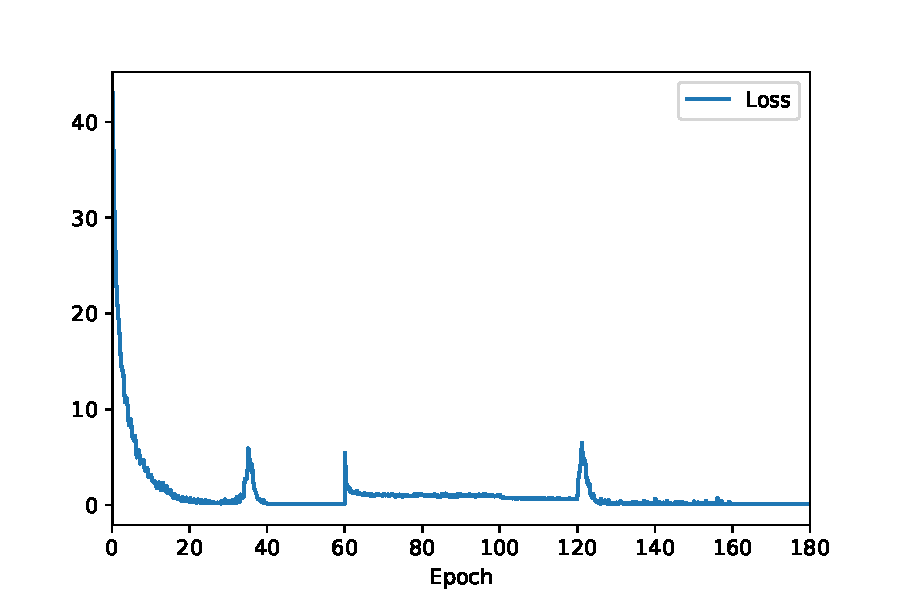
\includegraphics[width=0.6\textwidth]{loss}
\caption{交叉熵误差随着迭代次数变化曲线}
\label{fig:loss}
\end{figure}

\subsection{测试结果可视化}

图\ref{fig:testvis}是测试结果的可视化,左边一列是查询图片,每一张查询图片相应的右边一行是从测试库中挑选出来的图片,有红色边框的图片代表该人物标签与相应的查询图片人物标签不一致。

\begin{figure}
\centering
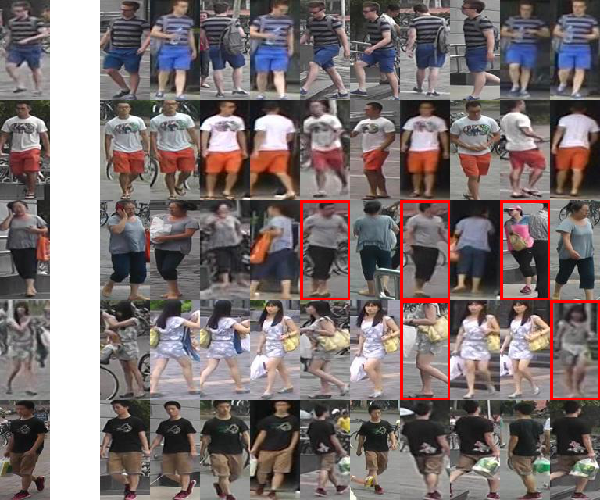
\includegraphics[width=0.7\textwidth]{vis3}
\caption{测试结果可视化}
\label{fig:testvis}
\end{figure}

\begin{table}[h!]
    \centering
    \caption{Market1501数据集测试结果}
    \label{tab:test}
    \begin{tabularx}{\textwidth}{XXXX}
    \toprule
               & mAP   & Rank1 & Rank10 \\ \midrule
    论文中显示  & 77.3  & 92.4  & 97.9   \\
    复现结果    & 71.1  & 86.2  & 93.4   \\ \bottomrule
    \end{tabularx}
\end{table}

\begin{table}[h!]
    \centering
    \caption{学习后选择的部署方案}
    \label{tab:rlresult}
    \begin{tabularx}{\textwidth}{XXX}
    \toprule
    方案               & 频次  & 占比      \\ \midrule
    (1, 2, 7, 10, 14) & 190 & 65.97\% \\
    (1, 2, 7, 10, 13) & 78  & 27.08\% \\
    (1, 2, 7, 9, 14)  & 18  & 6.15\%  \\
    (1, 3, 7, 10, 14) & 1   & 0.35\%  \\
    (0, 2, 7, 10, 14) & 1   & 0.35\%  \\ \bottomrule
    \end{tabularx}
\end{table}

\section{强化学习算法}

\subsection{学习后选择的部署方案}

表\ref{tab:rlresult}为经过强化学习训练后的智能体在应对各种状态时,最有可能采取的行动统计。其中方案(1, 2, 7, 10, 14)表示摄像头ID分别为1, 2, 7, 10, 14的部署方案,在该方案下的监控画面如图\ref{fig:rlresult}所示。从图中可以看到,从每一组内选取的摄像头光线充足、画面清晰、角度端正、视野范围宽阔,是一个比较好的摄像头部署方案。

\begin{figure}
\centering
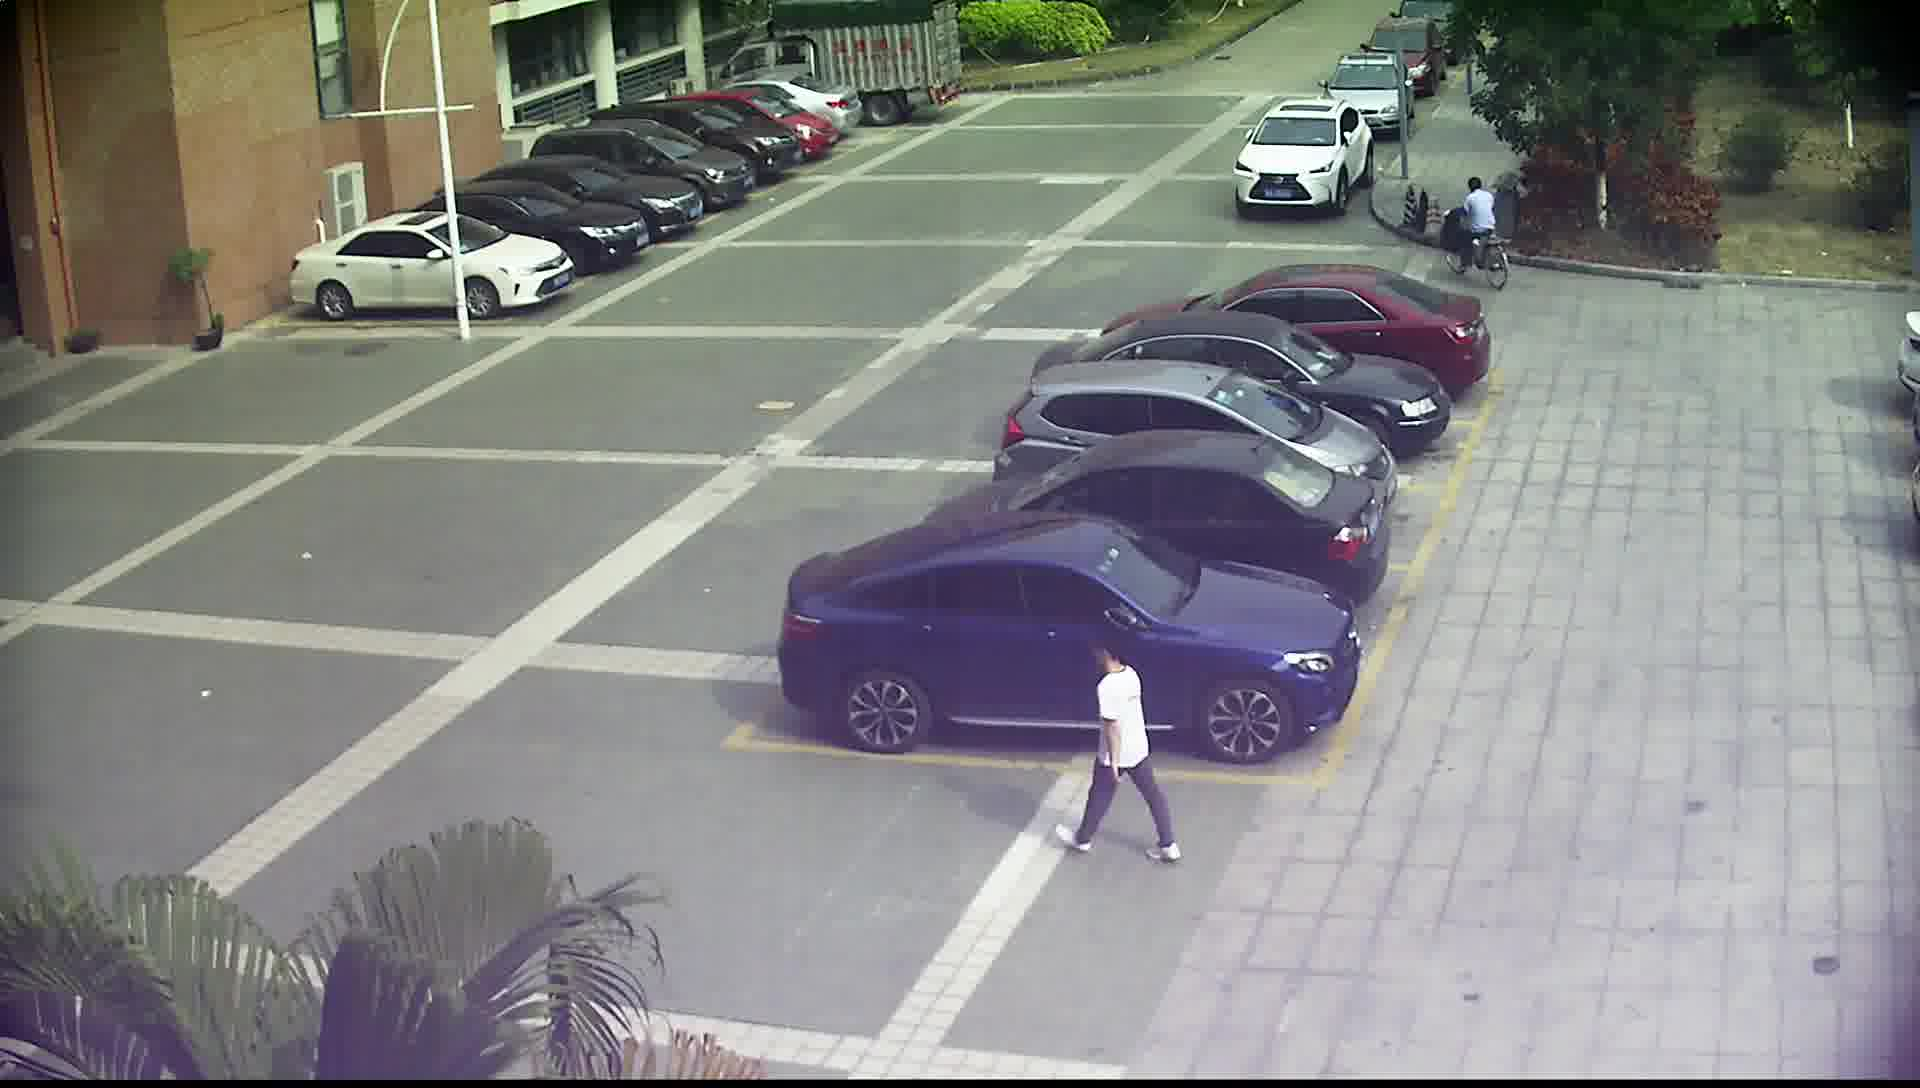
\includegraphics[width=0.3\textwidth]{1-2}
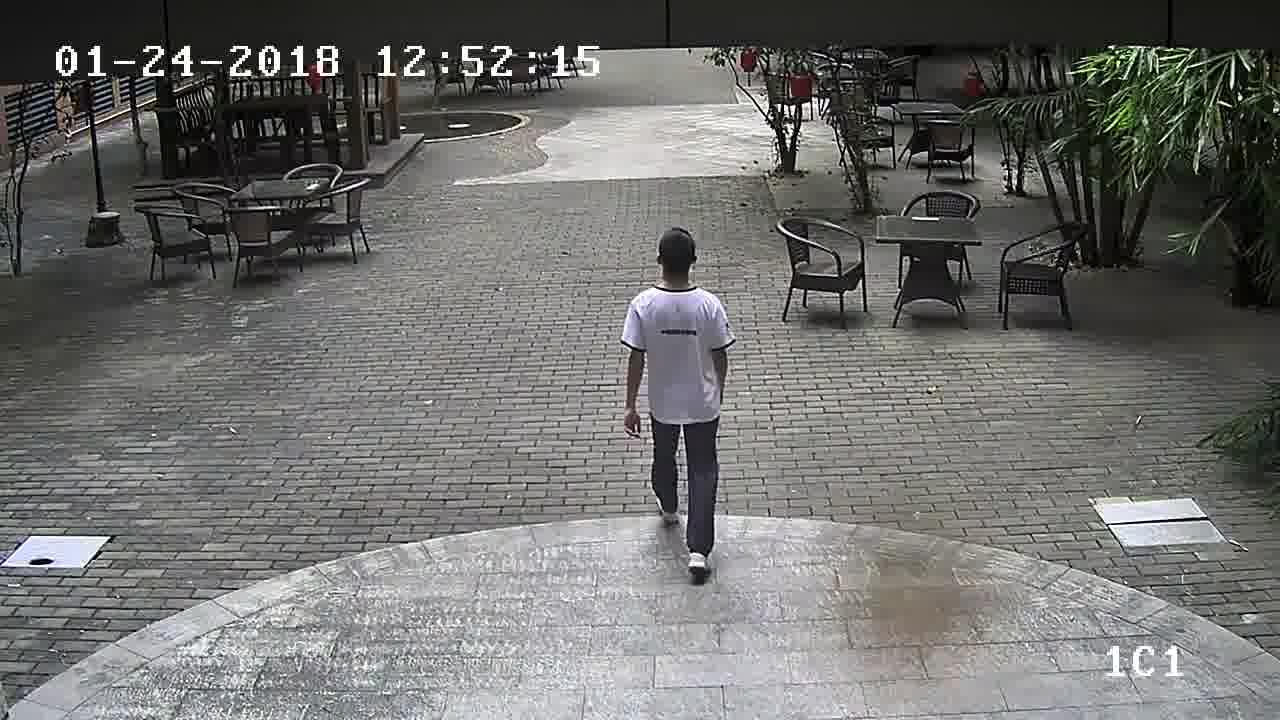
\includegraphics[width=0.3\textwidth]{1-4}\\
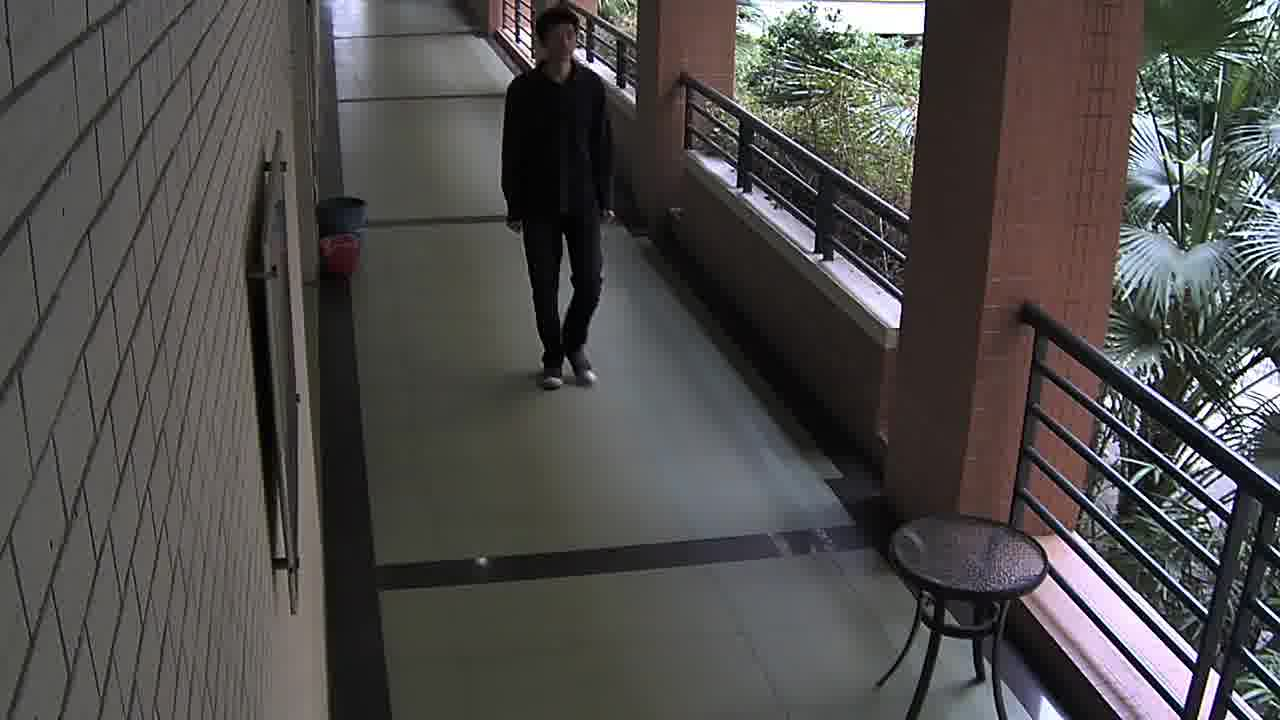
\includegraphics[width=0.3\textwidth]{2-3}
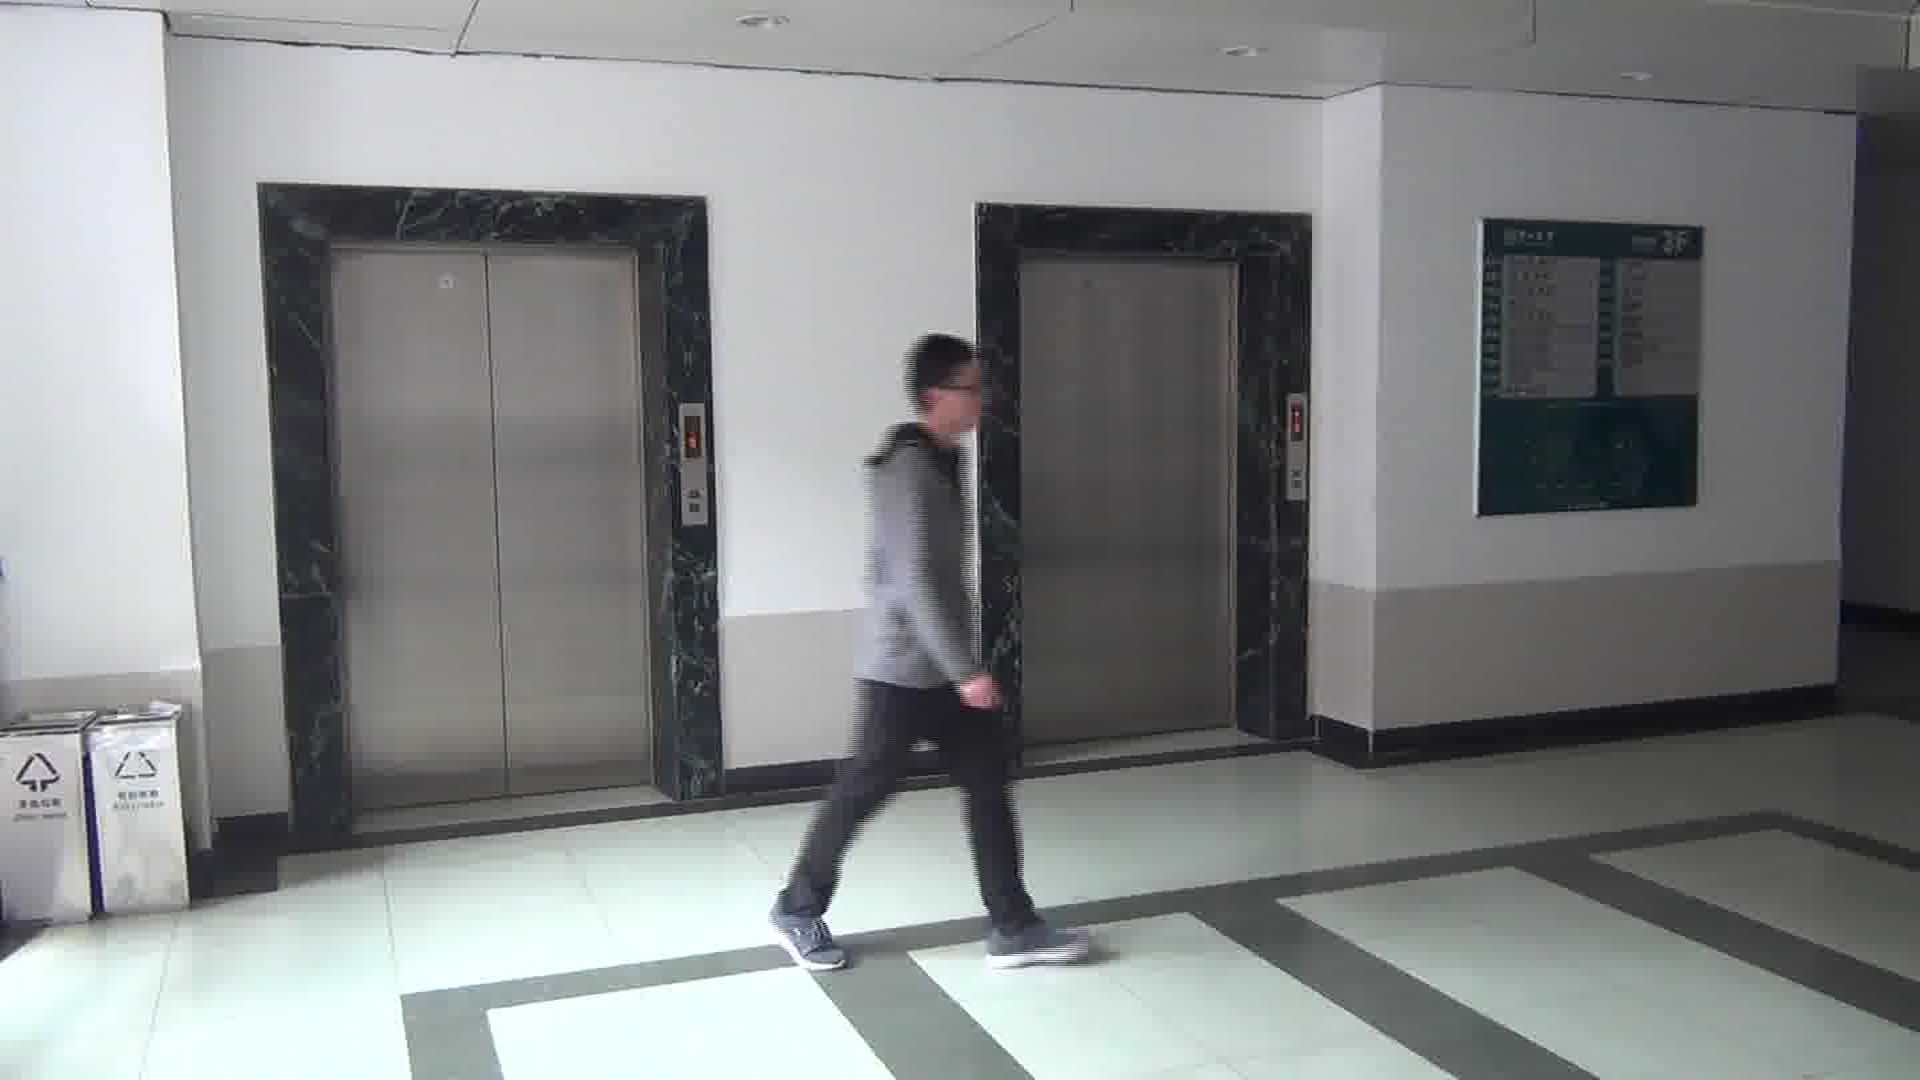
\includegraphics[width=0.3\textwidth]{3-2}
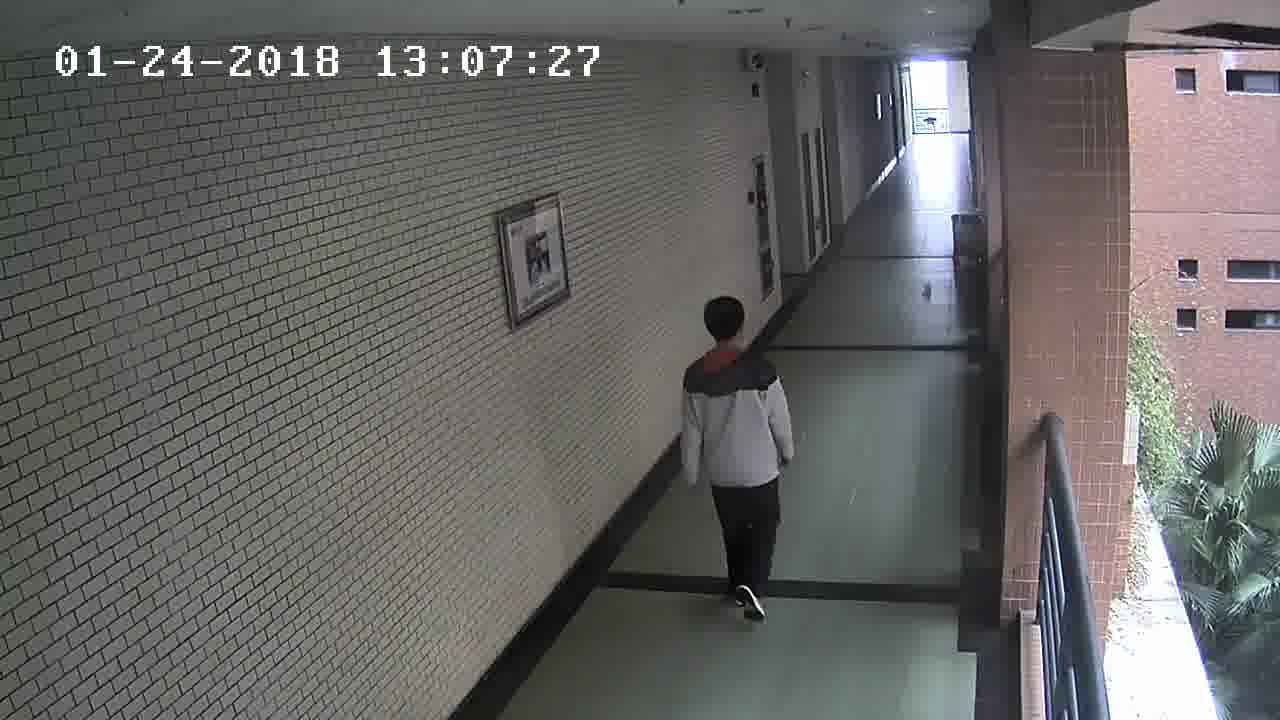
\includegraphics[width=0.3\textwidth]{3-6}
\caption{最优部署方案}
\label{fig:rlresult}
\end{figure}

假设智能体经过强化学习训练,对当前环境有了了解之后,采用贪心的策略,即无论当前处于什么状态,都采取使得长期价值最高的动作。基于此假设,表\ref{tab:rlresult}显示,在所有可能的状态中,智能体处于其中的$2/3$的状态下时都会一次性地转入之前讨论的(1, 2, 7, 10, 14)这个最优状态。处于其余接近$1/3$的状态下时会转入(1, 2, 7, 10, 13)这个次优状态,可以看出,此方案与最优方案之间的区别,仅仅在于最后一组的摄像头的选择,而经过检查,该摄像头的成像质量也比较优秀。与此同时,当智能体处于该次优方案的状态时,长期价值最高的动作是转入最优方案状态。同时剩余的三种状态也会马上转入最优方案状态。因此可以得出结论:无论智能体当前处于什么状态,至多经过两步,即可到达最优状态。

\section{分布式CPU训练}

\subsection{与单机的比较}

在天河二号上

单机CPU训练:5821 s/epoch

单机GPU训练:326 s/epoch

2节点多CPU训练:3016 s/epoch

4节点多CPU训练:1536 s/epoch

5节点多CPU训练:1219 s/epoch

\subsection{与GPU的比较}

batch size、学习率、epoch数、准确率